% =============================================================================
%  Diplomado en Data Science Aplicada con Python para la Toma de Decisiones
%  Clase 20: Interpretacion de Clusters, K-Means 3D y Pipelines
%  Arca Continental Ecuador | UDLA
%
%  Compilar: pdflatex -shell-escape presentacion.tex (x2 para refs)
% =============================================================================
\documentclass[aspectratio=169, 11pt]{beamer}

\usepackage[T1]{fontenc}
\usepackage[utf8]{inputenc}
\usepackage[spanish,es-noshorthands]{babel}
\usepackage{FiraSans}
\usepackage{FiraMono}
\renewcommand{\familydefault}{\sfdefault}
\usepackage{graphicx}
\usepackage{tikz}
\usetikzlibrary{arrows.meta, positioning, shapes.geometric, shapes.misc,
  calc, fit, decorations.pathreplacing, backgrounds}
\usepackage{fontawesome5}
\usepackage{minted}
\usepackage{tcolorbox}
\tcbuselibrary{minted, skins, breakable}
\usepackage{booktabs}
\usepackage{colortbl}
\usepackage{multicol}
\usepackage{hyperref}
\usepackage{calc}
\usepackage{amsmath}

\definecolor{arcaRed}{HTML}{C82B40}
\definecolor{arcaDark}{HTML}{6B1525}
\definecolor{udlaCrimson}{HTML}{A31545}
\definecolor{arcaGray}{HTML}{F5F5F5}
\definecolor{arcaLightGray}{HTML}{EBEBEB}
\definecolor{textDark}{HTML}{2D2D2D}
\definecolor{textMuted}{HTML}{6B7280}
\definecolor{codeGreen}{HTML}{16A34A}
\definecolor{codeBlue}{HTML}{2563EB}
\definecolor{codeOrange}{HTML}{EA580C}
\definecolor{codePurple}{HTML}{7C3AED}

\usetheme{default}
\usecolortheme{default}
\setbeamertemplate{navigation symbols}{}
\setbeamertemplate{footline}{}
\setbeamertemplate{headline}{}
\setbeamercolor{normal text}{fg=textDark}
\setbeamercolor{frametitle}{fg=arcaRed, bg=white}
\setbeamercolor{title}{fg=white}
\setbeamercolor{subtitle}{fg=white!85}
\setbeamercolor{author}{fg=white!80}
\setbeamercolor{date}{fg=white!70}
\setbeamercolor{item}{fg=arcaRed}
\setbeamercolor{subitem}{fg=arcaDark}
\setbeamercolor{block title}{fg=white, bg=arcaRed}
\setbeamercolor{block body}{fg=textDark, bg=arcaGray}
\setbeamercolor{block title alerted}{fg=white, bg=codeOrange}
\setbeamercolor{block body alerted}{fg=textDark, bg=arcaGray}
\setbeamercolor{block title example}{fg=white, bg=codeGreen}
\setbeamercolor{block body example}{fg=textDark, bg=arcaGray}
\setbeamercolor{section in toc}{fg=arcaDark}
\setbeamerfont{frametitle}{size=\Large, series=\bfseries}
\setbeamerfont{title}{size=\huge, series=\bfseries}
\setbeamerfont{subtitle}{size=\large}
\setbeamerfont{author}{size=\normalsize}
\setbeamerfont{date}{size=\small}
\setbeamerfont{block title}{size=\normalsize, series=\bfseries}
\setbeamerfont{footnote}{size=\tiny}
\setbeamertemplate{itemize item}{\scriptsize\raise1.5pt\hbox{\color{arcaRed}$\blacktriangleright$}}
\setbeamertemplate{itemize subitem}{\scriptsize\raise1pt\hbox{\color{arcaDark}$\bullet$}}
\setbeamertemplate{enumerate items}[default]
\setbeamercolor{enumerate item}{fg=arcaRed}

\setbeamertemplate{headline}{%
  \begin{tikzpicture}[remember picture, overlay]
    \fill[arcaDark] (current page.north west) rectangle
      ([yshift=-0.7cm]current page.north east);
    \node[anchor=west, inner sep=0pt] at
      ([xshift=0.6cm, yshift=-0.35cm]current page.north west)
      {
\includegraphics[height=0.45cm]{../logo_udla_white.png}};
    \node[anchor=east, inner sep=0pt] at
      ([xshift=-0.6cm, yshift=-0.35cm]current page.north east)
      {
\includegraphics[height=0.45cm]{../ArcaContinental_white.png}};
  \end{tikzpicture}%
  \vspace{0.7cm}%
}

\setbeamertemplate{footline}{%
  \begin{tikzpicture}[remember picture, overlay]
    \node[anchor=south east, font=\scriptsize\bfseries\color{arcaRed}] at
      ([xshift=-0.5cm, yshift=0.15cm]current page.south east)
      {\insertframenumber};
  \end{tikzpicture}%
  \vspace{0.3cm}%
}

\setbeamertemplate{frametitle}{%
  \vspace{0.25cm}%
  \usebeamerfont{frametitle}\usebeamercolor[fg]{frametitle}\insertframetitle%
  \par\vspace{2pt}%
  \begin{tikzpicture}
    \fill[arcaRed] (0,0) rectangle (3cm, 1.5pt);
    \fill[arcaLightGray] (3cm,0) rectangle (\textwidth, 0.5pt);
  \end{tikzpicture}%
  \vspace{0.1cm}%
}

\newtcblisting{pyblock}[1][]{%
  listing engine=minted, minted language=python, minted style=friendly,
  minted options={fontsize=\small, linenos=false, breaklines=true, python3=true},
  colback=arcaGray, colframe=arcaRed, left=4pt, right=4pt, top=4pt, bottom=4pt,
  boxrule=0pt, leftrule=3pt, arc=2pt, listing only, #1}

\newtcblisting{outputblock}[1][]{%
  listing engine=minted, minted language=text, minted style=bw,
  minted options={fontsize=\small, breaklines=true},
  colback=white, colframe=arcaLightGray, left=4pt, right=4pt, top=4pt, bottom=4pt,
  boxrule=0.5pt, arc=2pt, listing only,
  title={\small\faTerminal\hspace{6pt}Output}, coltitle=textMuted,
  fonttitle=\small\ttfamily, colbacktitle=white, #1}

\newcommand{\sectionframe}[2]{%
  \begingroup
  \setbeamertemplate{headline}{}%
  \setbeamertemplate{footline}{}%
  \begin{frame}[plain, noframenumbering]
    \begin{tikzpicture}[remember picture, overlay]
      \fill[arcaRed] (current page.south west) rectangle (current page.north east);
      \node[anchor=center, text=white, font=\Huge\bfseries, text width=12cm,
            align=center] at ([yshift=0.5cm]current page.center) {#1};
      \node[anchor=center, text=white!80, font=\large, text width=10cm,
            align=center] at ([yshift=-0.8cm]current page.center) {#2};
    \end{tikzpicture}
  \end{frame}
  \endgroup
}

\title{Diplomado en Data Science Aplicada\\con Python para la Toma de Decisiones}
\subtitle{Clase 20: Interpretaci\'on de Clusters, DBSCAN y Pipelines}
\author{Carlos Enrique Mosquera Trujillo}
\date{29 de Abril, 2026}

\begin{document}

% ── PORTADA ──────────────────────────────────────────────────────────────────
{
\setbeamertemplate{headline}{}
\setbeamertemplate{footline}{}
\begin{frame}[plain, noframenumbering]
  \begin{tikzpicture}[remember picture, overlay]
    \fill[arcaDark] (current page.south west) rectangle (current page.north east);
    \fill[arcaRed] ([yshift=-3.5cm]current page.north west) rectangle
      ([yshift=-4.2cm]current page.north east);
    \node[anchor=west, inner sep=0pt] at
      ([xshift=1cm, yshift=-1.5cm]current page.north west)
      {
\includegraphics[height=1cm]{../logo_udla_white.png}};
    \node[anchor=east, inner sep=0pt] at
      ([xshift=-1cm, yshift=-1.5cm]current page.north east)
      {
\includegraphics[height=1cm]{../ArcaContinental_white.png}};
  \end{tikzpicture}
  \vspace{2.5cm}
  \begin{center}
    {\usebeamerfont{title}\usebeamercolor[fg]{title}\inserttitle\par}
    \vspace{0.4cm}
    {\usebeamerfont{subtitle}\usebeamercolor[fg]{subtitle}\insertsubtitle\par}
    \vspace{0.6cm}
    {\usebeamerfont{author}\usebeamercolor[fg]{author}\insertauthor\par}
    \vspace{0.15cm}
    {\usebeamerfont{date}\usebeamercolor[fg]{date}\insertdate\par}
  \end{center}
\end{frame}
}

% ── M\'ODULO 4 ─────────────────────────────────────────────────────────────────
{
\setbeamertemplate{headline}{}
\setbeamertemplate{footline}{}
\begin{frame}[plain, noframenumbering]
  \begin{tikzpicture}[remember picture, overlay]
    \fill[arcaDark] (current page.south west) rectangle (current page.north east);
    \node[anchor=center, text=white, font=\Large\bfseries, text width=12cm,
          align=center] at ([yshift=1cm]current page.center)
      {M\'odulo 4 --- clase 7};
    \node[anchor=center, text=white!90, font=\huge\bfseries, text width=12cm,
          align=center] at ([yshift=-0.3cm]current page.center)
      {Machine Learning};
  \end{tikzpicture}
\end{frame}
}

% ── ROADMAP ─────────────────────────────────────────────────────────────────
\begin{frame}[shrink=22]{Hoja de Ruta de Hoy}
  \vspace{-4pt}
  \begin{center}
  \begin{tikzpicture}[
    node distance=0.35cm,
    roadstep/.style={rectangle, rounded corners=4pt, draw=arcaRed, fill=arcaRed!8,
                 minimum width=11cm, minimum height=0.65cm,
                 font=\footnotesize\bfseries\color{arcaDark}, align=left,
                 text width=10cm, inner sep=6pt},
    num/.style={circle, fill=arcaRed, text=white, font=\scriptsize\bfseries,
                minimum size=0.5cm, inner sep=0pt},
  ]
    \node[roadstep] (s0) {\hspace{0.8cm}Retomar: interpretar los 5 segmentos de clientes (2D)};
    \node[roadstep, below=of s0] (s1) {\hspace{0.8cm}K-Means 3D: agregar edad, StandardScaler, scatter\_3d};
    \node[roadstep, below=of s1] (s2) {\hspace{0.8cm}DBSCAN: cuando K-Means falla (lunas, c\'irculos, outliers)};
    \node[roadstep, below=of s2] (s3) {\hspace{0.8cm}?`Y el cliente nuevo? De clustering a clasificaci\'on};
    \node[roadstep, below=of s3] (s4) {\hspace{0.8cm}Ejercicio: descubrir especies sin etiquetas (Iris)};
    \node[roadstep, below=of s4] (s5) {\hspace{0.8cm}Pipelines de sklearn: encadenar preprocesamiento + modelo};
    \node[roadstep, below=of s5] (s6) {\hspace{0.8cm}Pipeline + Cross-Validation + GridSearchCV};

    \node[num] at ([xshift=0.45cm]s0.west) {1};
    \node[num] at ([xshift=0.45cm]s1.west) {2};
    \node[num] at ([xshift=0.45cm]s2.west) {3};
    \node[num] at ([xshift=0.45cm]s3.west) {4};
    \node[num] at ([xshift=0.45cm]s4.west) {5};
    \node[num] at ([xshift=0.45cm]s5.west) {6};
    \node[num] at ([xshift=0.45cm]s6.west) {7};
  \end{tikzpicture}
  \end{center}
\end{frame}

% =============================================================================
%  BLOQUE A: INTERPRETAR CLUSTERS 2D
% =============================================================================
\sectionframe{Interpretar los Clusters}{De n\'umeros a decisiones de negocio}

\begin{frame}{El Cluster No Sirve Sin Interpretaci\'on}
  \vspace{-4pt}
  {\footnotesize\color{arcaDark}\bfseries
    En la clase pasada encontramos 5 segmentos con K-Means. Pero
    ``cluster 0, 1, 2, 3, 4'' no le dice \textbf{nada} a un gerente.
    Hoy convertimos n\'umeros en \textbf{acciones}.}

  \vspace{6pt}
  {\footnotesize
  \begin{itemize}\setlength{\itemsep}{5pt}
    \item[{\color{arcaRed}\scriptsize\faArrowRight}]
      \textbf{Paso 1: Perfilar} --- calcular promedios de cada variable
      por cluster. ?`Qu\'e tiene de especial cada grupo?
    \item[{\color{arcaRed}\scriptsize\faArrowRight}]
      \textbf{Paso 2: Nombrar} --- darle un nombre que un gerente entienda:
      ``Premium'', ``Ahorradores VIP'', no ``cluster 3''.
    \item[{\color{codeGreen}\scriptsize\faArrowRight}]
      \textbf{Paso 3: Recomendar} --- cada segmento recibe una
      estrategia diferente. Eso es el valor real.
  \end{itemize}
  }

  \vspace{4pt}
  \begin{tcolorbox}[colback=arcaGray, colframe=arcaRed, boxrule=0.5pt, arc=2pt,
    left=6pt, right=6pt, top=4pt, bottom=4pt]
    {\scriptsize\color{arcaDark}
    \faKey\hspace{4pt}\textbf{Un cluster sin interpretaci\'on es in\'util.}
    El valor no est\'a en el algoritmo, sino en la \textbf{acci\'on}
    que tomas con cada grupo.}
  \end{tcolorbox}
\end{frame}

\begin{frame}[fragile,shrink=10]{Perfilar: Promedios por Cluster}
  \vspace{-4pt}
  {\footnotesize\color{arcaDark}\bfseries
    El primer paso: ?`qu\'e promedio de ingreso, gasto y edad tiene
    cada cluster?}

  \vspace{4pt}
  \begin{pyblock}
perfil = df.groupby("cluster")[["Age", "income", "spending"]]\
    .agg(["mean", "std", "count"])
perfil = perfil.round(1)
perfil
  \end{pyblock}

  \vspace{4pt}
  {\scriptsize\color{arcaDark}
    \faKey\hspace{4pt} La \textbf{media} dice el valor t\'ipico.
    La \textbf{std} dice qu\'e tan homog\'eneo es el grupo ---
    si es baja, los miembros se parecen entre s\'i.
    El \textbf{count} dice cu\'antos clientes hay.}
\end{frame}

\begin{frame}[shrink=18]{Los 5 Segmentos con Nombres de Negocio}
  \vspace{-4pt}
  \begin{center}
    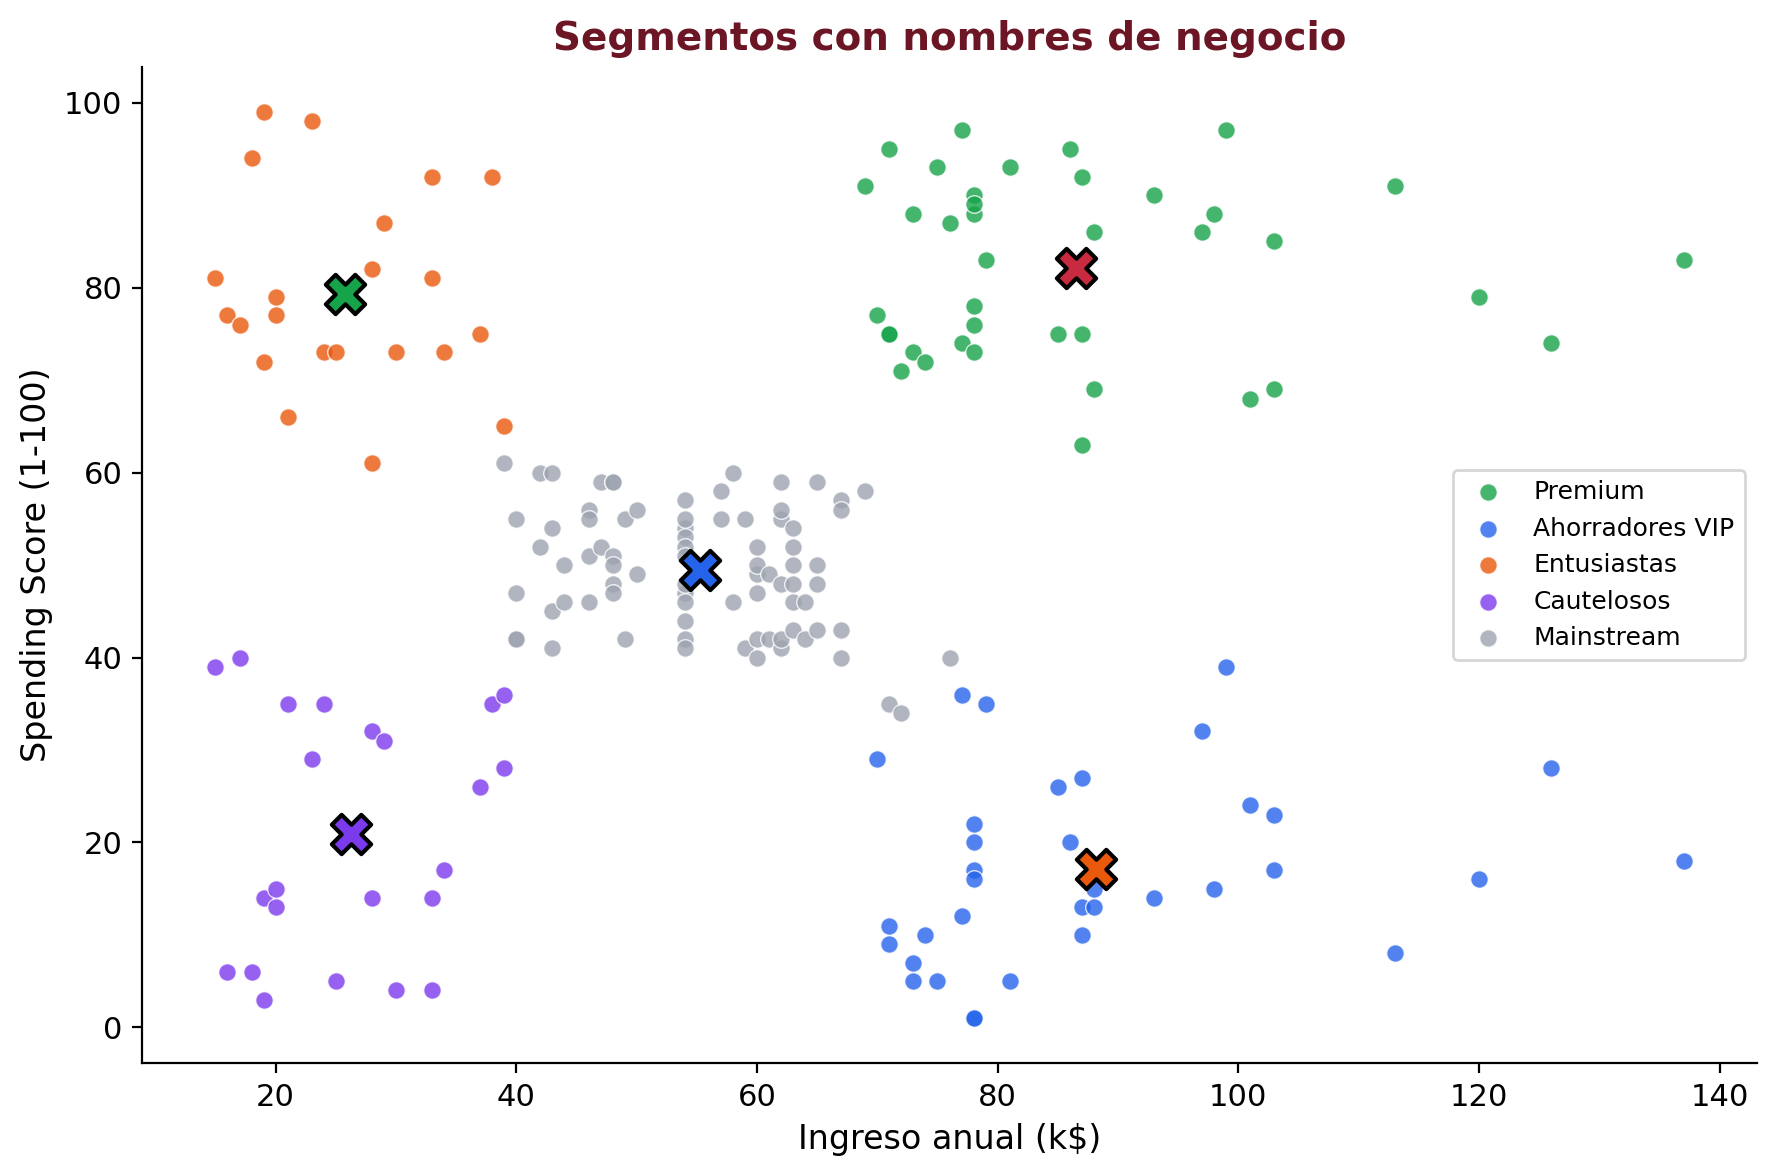
\includegraphics[width=0.78\textwidth]{fig_segmentos_nombres.png}
  \end{center}

  \vspace{-2pt}
  {\scriptsize\color{textMuted}
    \faLightbulb\hspace{4pt} Ahora cada punto tiene un nombre que un gerente
    entiende. No ``cluster 3'' sino ``Ahorradores VIP'' --- personas con
    alto ingreso que no gastan. \textbf{La oportunidad m\'as grande.}}
\end{frame}

\begin{frame}[shrink=18]{Barras: Ingreso vs Gasto por Segmento}
  \vspace{-4pt}
  \begin{center}
    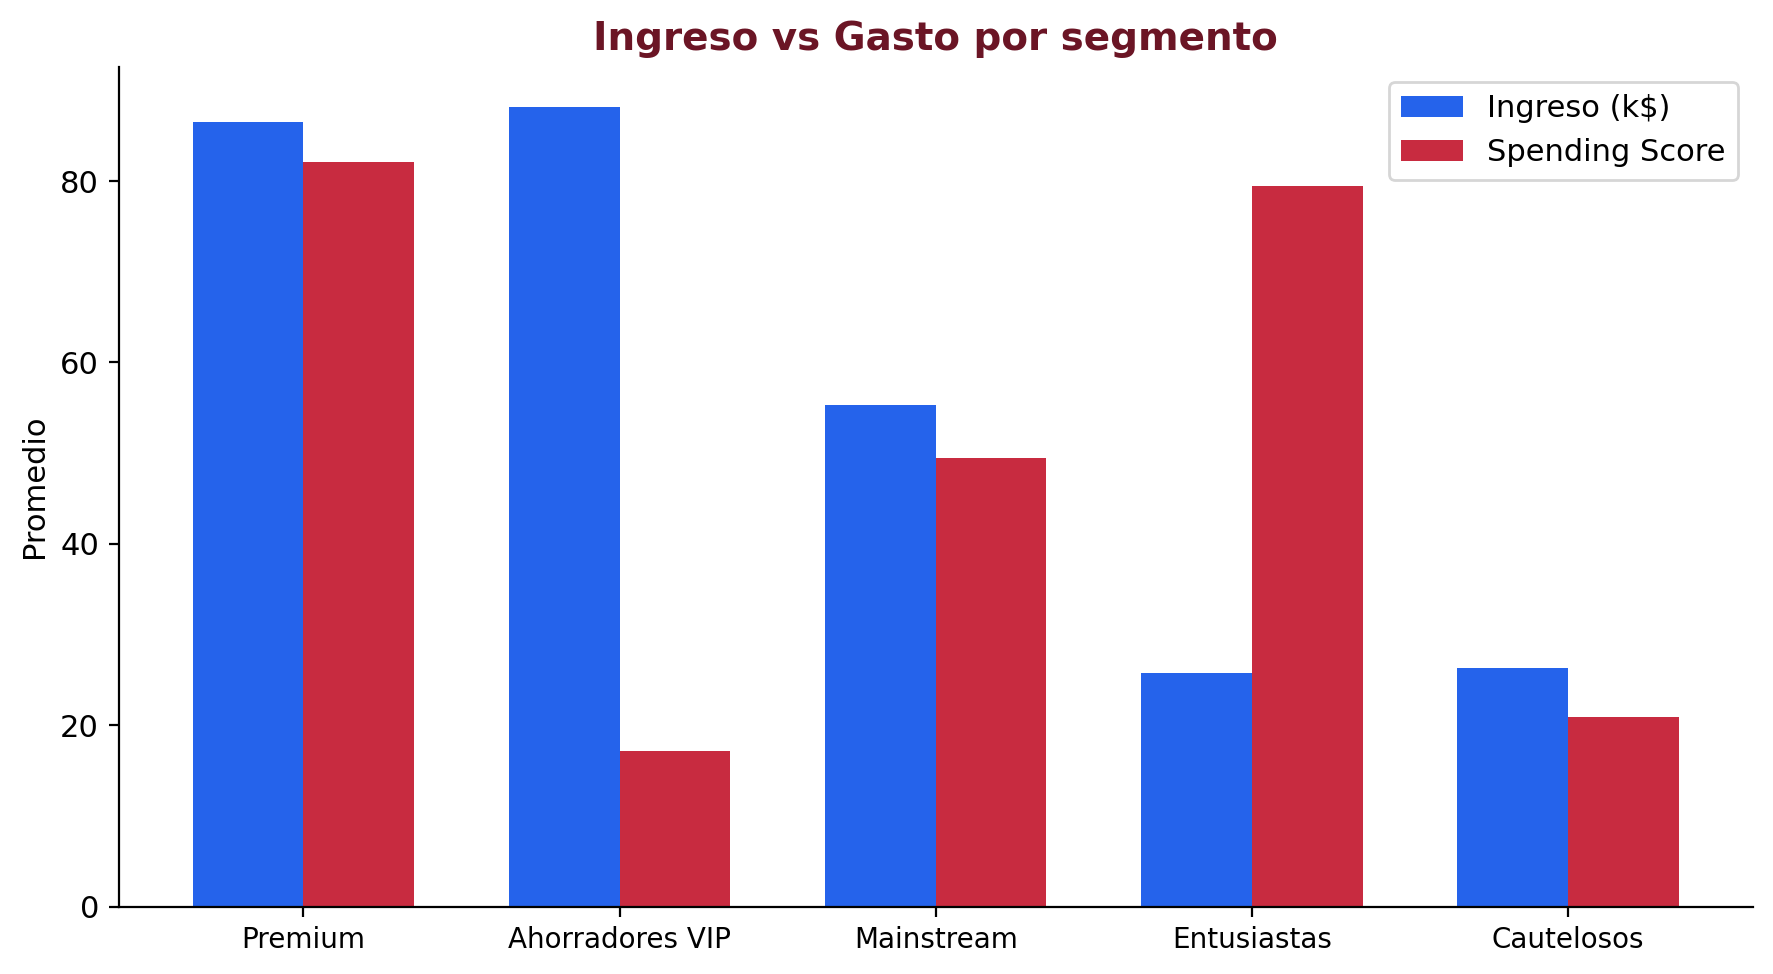
\includegraphics[width=0.78\textwidth]{fig_barras_segmento.png}
  \end{center}

  \vspace{-2pt}
  {\scriptsize\color{textMuted}
    \faLightbulb\hspace{4pt} La \textbf{brecha} entre barras azules (ingreso)
    y rojas (gasto) revela la oportunidad. Ahorradores VIP: ganan mucho,
    gastan poco. Entusiastas: gastan m\'as de lo que su ingreso sugiere.}
\end{frame}

\begin{frame}[shrink=18]{Radar Chart: La ``Forma'' de Cada Segmento}
  \vspace{-4pt}
  \begin{center}
    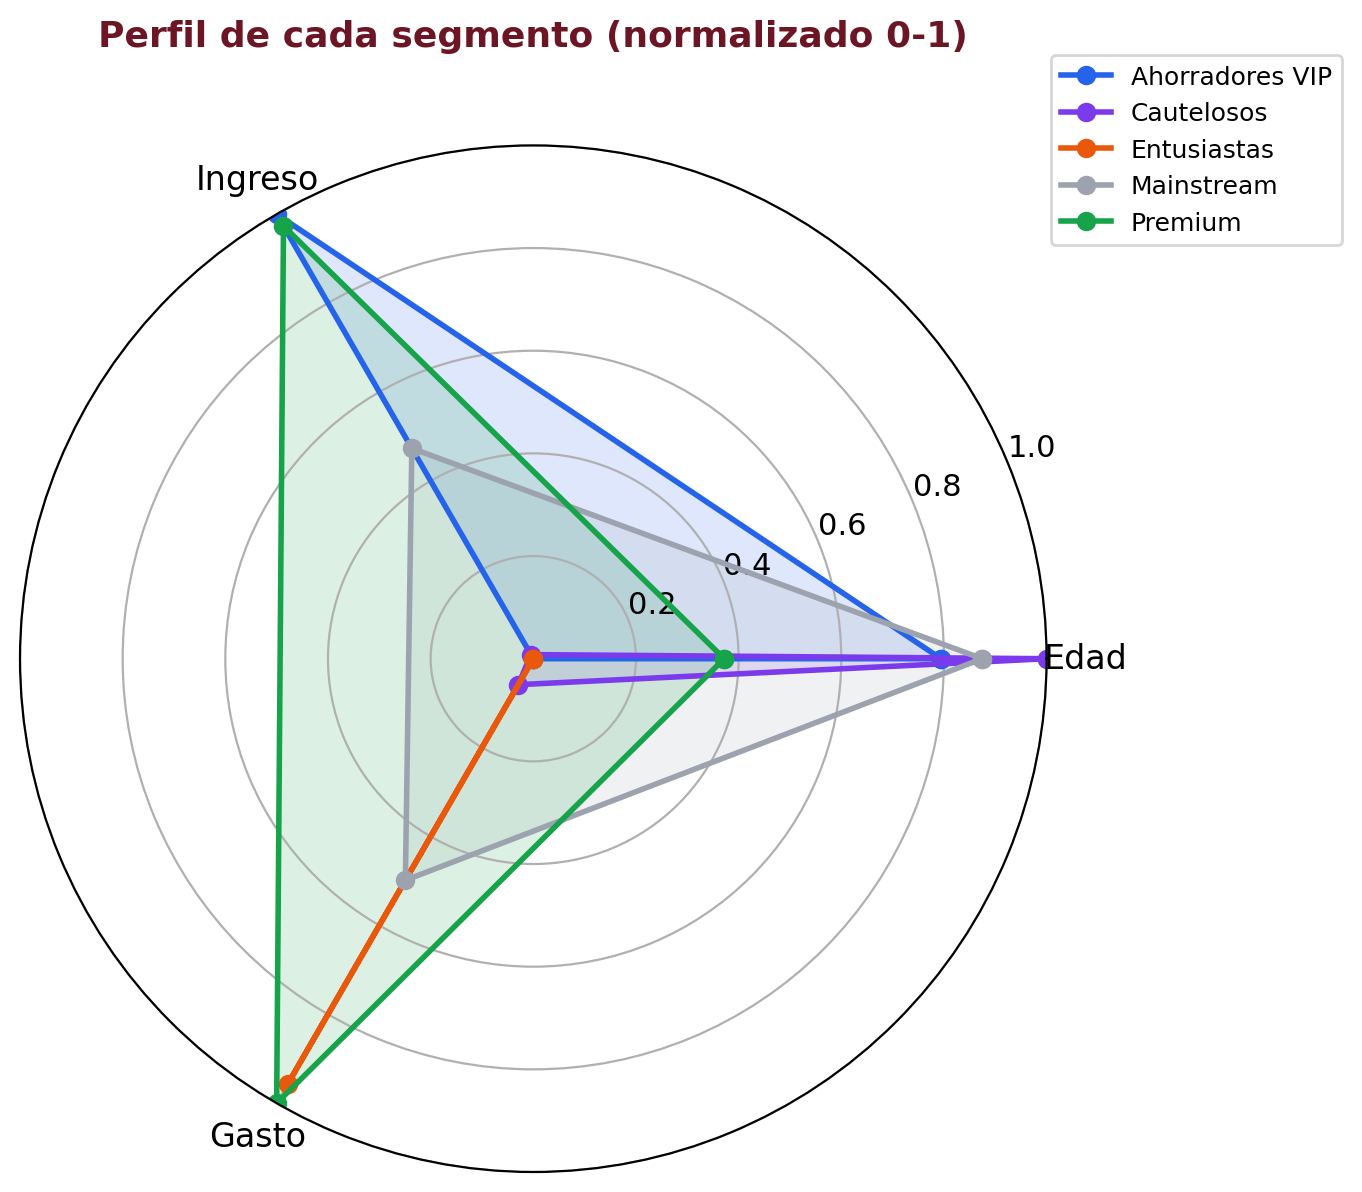
\includegraphics[width=0.58\textwidth]{fig_radar.png}
  \end{center}

  \vspace{-2pt}
  {\scriptsize\color{textMuted}
    \faLightbulb\hspace{4pt} El radar chart muestra de un vistazo el
    perfil de cada segmento. Los Premium tienen ingreso y gasto altos.
    Los Cautelosos tienen todo bajo. Ideal para presentaciones ejecutivas.}
\end{frame}

\begin{frame}[shrink=5]{Recomendaciones de Negocio por Segmento}
  \vspace{-4pt}
  {\scriptsize
  \begin{tabular}{@{}p{2.2cm}p{3cm}p{5cm}p{1.5cm}@{}}
    \toprule
    \textbf{Segmento} & \textbf{Perfil} & \textbf{Estrategia} & \textbf{Prioridad} \\
    \midrule
    \textbf{\color{codeGreen}Premium} & Ingreso alto, gasto alto & Lealtad exclusivo, productos premium, experiencias VIP & Retener \\
    \textbf{\color{codeBlue}Ahorradores VIP} & Ingreso alto, gasto bajo & Incentivar: descuentos, tarjeta, beneficios por compra & Activar \\
    \textbf{\color{codeOrange}Entusiastas} & Ingreso bajo, gasto alto & Proteger: son leales, sensibles al precio & Proteger \\
    \textbf{\color{codePurple}Cautelosos} & Ingreso bajo, gasto bajo & Comunicaci\'on b\'asica, ofertas masivas & Monitorear \\
    \textbf{Mainstream} & Ingreso y gasto medio & Upselling gradual hacia Premium o Entusiastas & Desarrollar \\
    \bottomrule
  \end{tabular}
  }

  \vspace{6pt}
  \begin{tcolorbox}[colback=arcaGray, colframe=arcaRed, boxrule=0.5pt, arc=2pt,
    left=6pt, right=6pt, top=4pt, bottom=4pt]
    {\scriptsize\color{arcaDark}
    \faKey\hspace{4pt}\textbf{La segmentaci\'on transforma datos en decisiones.}
    Sin K-Means, tratar\'iamos a los 200 clientes igual.
    Con K-Means, cada segmento recibe la estrategia correcta.}
  \end{tcolorbox}
\end{frame}

% =============================================================================
%  BLOQUE B: K-MEANS 3D
% =============================================================================
\sectionframe{K-Means en 3D}{Agregar edad como tercera variable}

\begin{frame}{?`Por Qu\'e Agregar Variables?}
  \vspace{-4pt}
  {\footnotesize\color{arcaDark}\bfseries
    Hasta ahora usamos solo ingreso y gasto. Pero la \textbf{edad}
    var\'ia entre segmentos. Si la incluimos, K-Means podr\'a
    encontrar grupos m\'as finos.}

  \vspace{6pt}
  {\footnotesize
  \begin{itemize}\setlength{\itemsep}{5pt}
    \item[{\color{arcaRed}\scriptsize\faExclamationTriangle}]
      \textbf{Problema de escala:} income va de 15 a 137, spending de 1 a 99,
      Age de 18 a 70. K-Means mide distancias --- la variable con
      valores m\'as grandes domina.
    \item[{\color{codeGreen}\scriptsize\faCheckCircle}]
      \textbf{Soluci\'on:} \texttt{StandardScaler} transforma cada variable
      para que tenga media 0 y desviaci\'on 1. Ahora las tres pesan igual.
    \item[{\color{codeBlue}\scriptsize\faArrowRight}]
      El K \'optimo puede \textbf{cambiar} al agregar variables.
      M\'as dimensiones = m\'as estructura posible.
  \end{itemize}
  }

  \vspace{4pt}
  {\scriptsize\color{textMuted}
    \faLightbulb\hspace{4pt} M\'as variables no siempre es mejor.
    A veces agregar variables ruidosas empeora la segmentaci\'on.
    Elegir las variables correctas es parte del trabajo.}
\end{frame}

\begin{frame}[fragile,shrink=10]{C\'odigo: Escalar y Aplicar K-Means 3D}
  \vspace{-4pt}
  \begin{pyblock}
from sklearn.preprocessing import StandardScaler

scaler = StandardScaler()
X_3d = scaler.fit_transform(df[["income", "spending", "Age"]])

# Verificar
print("Antes:", df[["income","spending","Age"]].std().round(1).tolist())
print("Despues:", pd.DataFrame(X_3d).std().round(2).tolist())
# -> [1.0, 1.0, 1.0]  Todas iguales!

km_3d = KMeans(n_clusters=6, random_state=42, n_init=10)
df["cluster_3d"] = km_3d.fit_predict(X_3d)
  \end{pyblock}

  \vspace{4pt}
  {\scriptsize\color{arcaDark}
    \faKey\hspace{4pt} Despu\'es de escalar, las tres variables tienen
    desviaci\'on est\'andar 1. K-Means las trata con igual importancia.}
\end{frame}

\begin{frame}[shrink=18]{Codo + Silhouette para 3 Variables}
  \vspace{-4pt}
  \begin{center}
    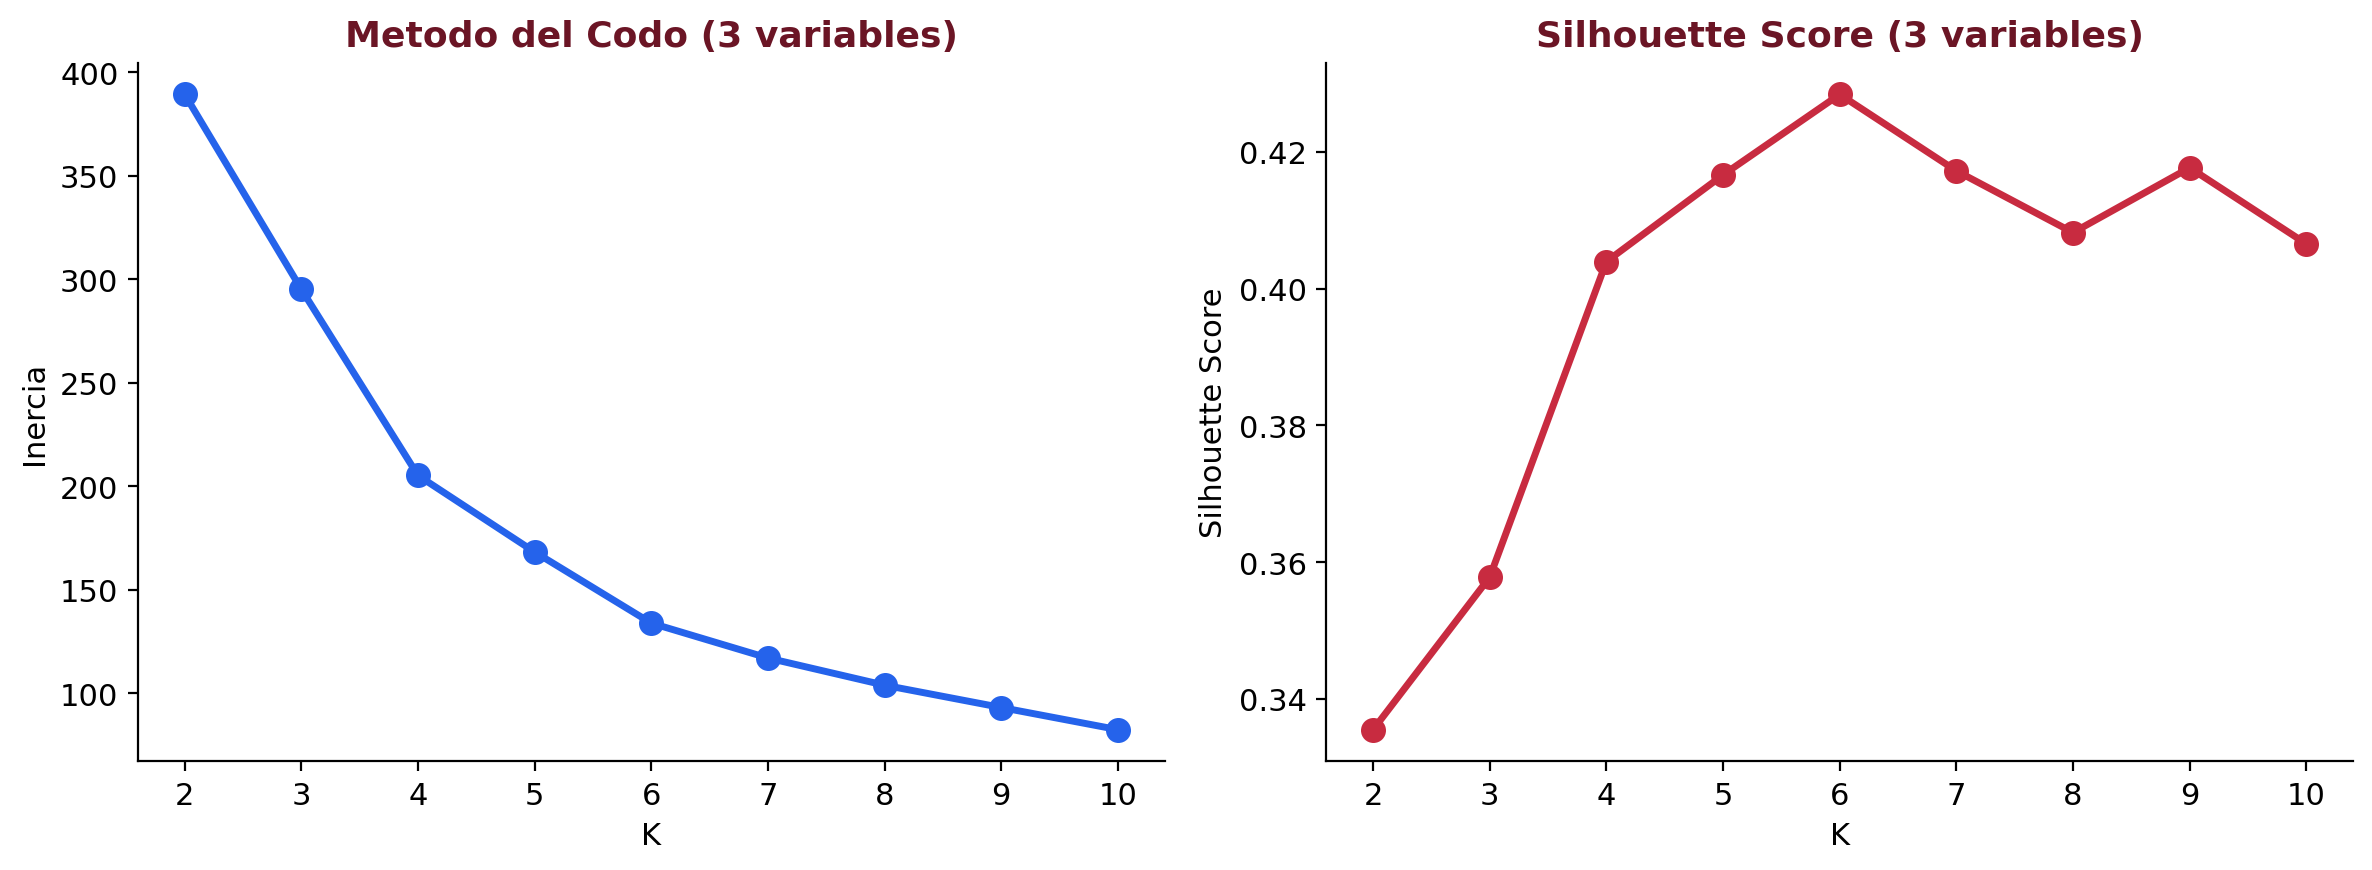
\includegraphics[width=0.88\textwidth]{fig_codo_silhouette_3d.png}
  \end{center}

  \vspace{-2pt}
  {\scriptsize\color{textMuted}
    \faLightbulb\hspace{4pt} Al agregar edad, el K \'optimo puede cambiar
    respecto a 2D. El codo y el Silhouette pueden sugerir un K distinto.
    Usar ambos m\'etodos da m\'as confianza.}
\end{frame}

\begin{frame}[fragile,shrink=10]{Scatter 3D Interactivo con Plotly}
  \vspace{-4pt}
  \begin{pyblock}
fig = px.scatter_3d(
    df, x="income", y="spending", z="Age",
    color=df["cluster_3d"].astype(str),
    title="Segmentacion 3D",
    labels={"income": "Ingreso (k$)",
            "spending": "Spending Score",
            "Age": "Edad"})
fig.update_layout(template="plotly_white")
fig.show()
  \end{pyblock}

  \vspace{4pt}
  {\scriptsize\color{arcaDark}
    \faMousePointer\hspace{4pt} \texttt{px.scatter\_3d} genera un gr\'afico
    que se puede \textbf{rotar} con el mouse. La tercera dimensi\'on
    permite ver separaciones invisibles en 2D.}
\end{frame}

\begin{frame}[shrink=18]{Heatmap: Perfil de Cada Cluster 3D}
  \vspace{-4pt}
  \begin{center}
    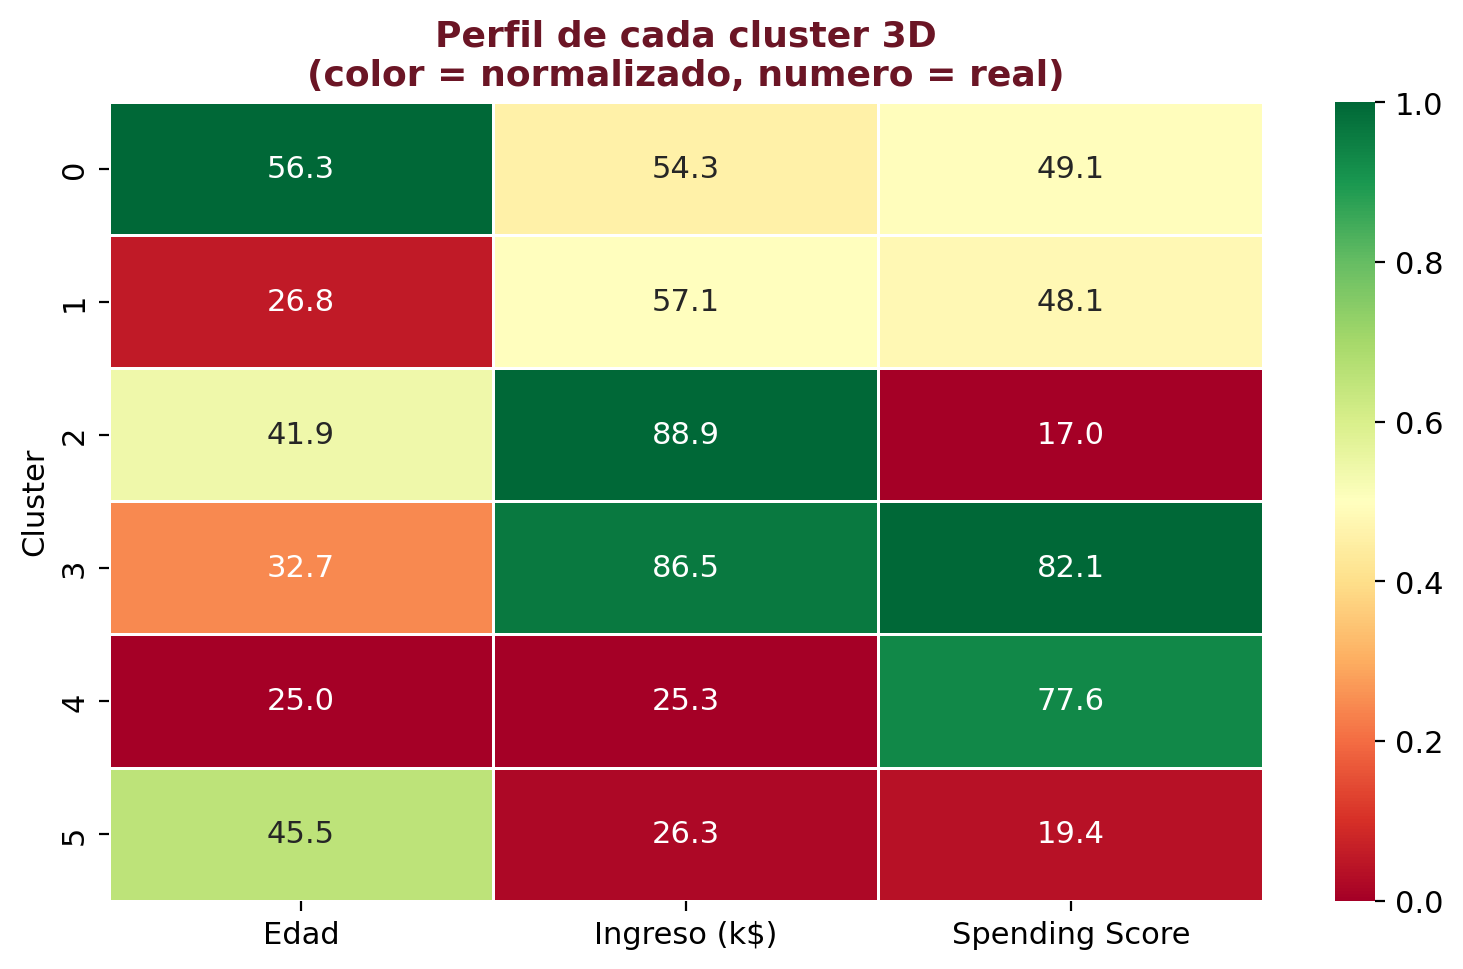
\includegraphics[width=0.68\textwidth]{fig_heatmap_3d.png}
  \end{center}

  \vspace{-2pt}
  {\scriptsize\color{textMuted}
    \faLightbulb\hspace{4pt} Verde = valor alto, rojo = valor bajo.
    Los n\'umeros son los valores reales. De un vistazo se identifica
    cada perfil: un cluster con edad alta + ingreso alto + gasto bajo
    es un ``jubilado ahorrador''.}
\end{frame}

\begin{frame}{2D vs 3D: ?`Qu\'e Cambi\'o?}
  \vspace{-4pt}
  {\footnotesize\color{arcaDark}\bfseries
    Al pasar de 2D a 3D, algunos segmentos originales se ``parten''
    por la edad:}

  \vspace{6pt}
  {\footnotesize
  \begin{itemize}\setlength{\itemsep}{5pt}
    \item[{\color{arcaRed}\scriptsize\faArrowRight}]
      El grupo ``Mainstream'' del centro puede dividirse en
      j\'ovenes y mayores.
    \item[{\color{arcaRed}\scriptsize\faArrowRight}]
      Dos clientes con el mismo ingreso y gasto pero edades
      muy diferentes ahora caen en clusters distintos.
    \item[{\color{codeGreen}\scriptsize\faArrowRight}]
      M\'as variables = segmentaci\'on m\'as fina, pero tambi\'en
      m\'as compleja de explicar.
  \end{itemize}
  }

  \vspace{4pt}
  \begin{tcolorbox}[colback=arcaGray, colframe=arcaRed, boxrule=0.5pt, arc=2pt,
    left=6pt, right=6pt, top=4pt, bottom=4pt]
    {\scriptsize\color{arcaDark}
    \faKey\hspace{4pt}\textbf{La decisi\'on depende del negocio:}
    si la edad importa para las campa\~nas, 3D es mejor.
    Si solo importa el gasto, 2D basta. No hay respuesta universal.}
  \end{tcolorbox}
\end{frame}

\begin{frame}[shrink=5]{Ejercicio 2: Nombrar los Segmentos 3D}
  \vspace{-4pt}
  {\footnotesize\color{arcaDark}\bfseries
    \faClock\hspace{4pt} 5 minutos:}

  \vspace{6pt}
  {\footnotesize
  \begin{enumerate}\setlength{\itemsep}{4pt}
    \item Miren el heatmap de la secci\'on anterior.
    \item Asignen un nombre de negocio a cada cluster usando las
      3 variables (edad, ingreso, gasto).
    \item Ejemplo: edad alta + ingreso alto + gasto bajo =
      ``Jubilado ahorrador''.
  \end{enumerate}
  }
\end{frame}

% =============================================================================
%  BLOQUE C: DBSCAN
% =============================================================================
\sectionframe{DBSCAN}{?`Y cuando K-Means falla?}

\begin{frame}{K-Means Asume Clusters Esf\'ericos}
  \vspace{-4pt}
  {\footnotesize\color{arcaDark}\bfseries
    K-Means funciona bien cuando los grupos son ``bolitas'' separadas.
    Pero los datos reales no siempre tienen esa forma.}

  \vspace{6pt}
  {\footnotesize
  \begin{itemize}\setlength{\itemsep}{5pt}
    \item[{\color{arcaRed}\scriptsize\faTimesCircle}]
      K-Means divide el espacio con \textbf{l\'ineas rectas}
      (diagramas de Voronoi). Si los clusters tienen forma de luna,
      espiral o anillo, \textbf{falla}.
    \item[{\color{arcaRed}\scriptsize\faTimesCircle}]
      K-Means necesita que \textbf{nosotros} elijamos $K$.
      Si no sabemos cu\'antos grupos hay, estamos adivinando.
    \item[{\color{arcaRed}\scriptsize\faTimesCircle}]
      K-Means \textbf{asigna todos los puntos} a alg\'un cluster.
      No detecta outliers --- un punto raro se fuerza dentro de
      un grupo al que no pertenece.
  \end{itemize}
  }

  \vspace{4pt}
  {\scriptsize\color{textMuted}
    \faArrowRight\hspace{4pt} Necesitamos un algoritmo que no asuma
    formas y que pueda decir ``este punto no pertenece a ning\'un grupo''.}
\end{frame}

\begin{frame}[shrink=22]{Cuando K-Means Falla --- Visual}
  \vspace{-4pt}
  \begin{center}
    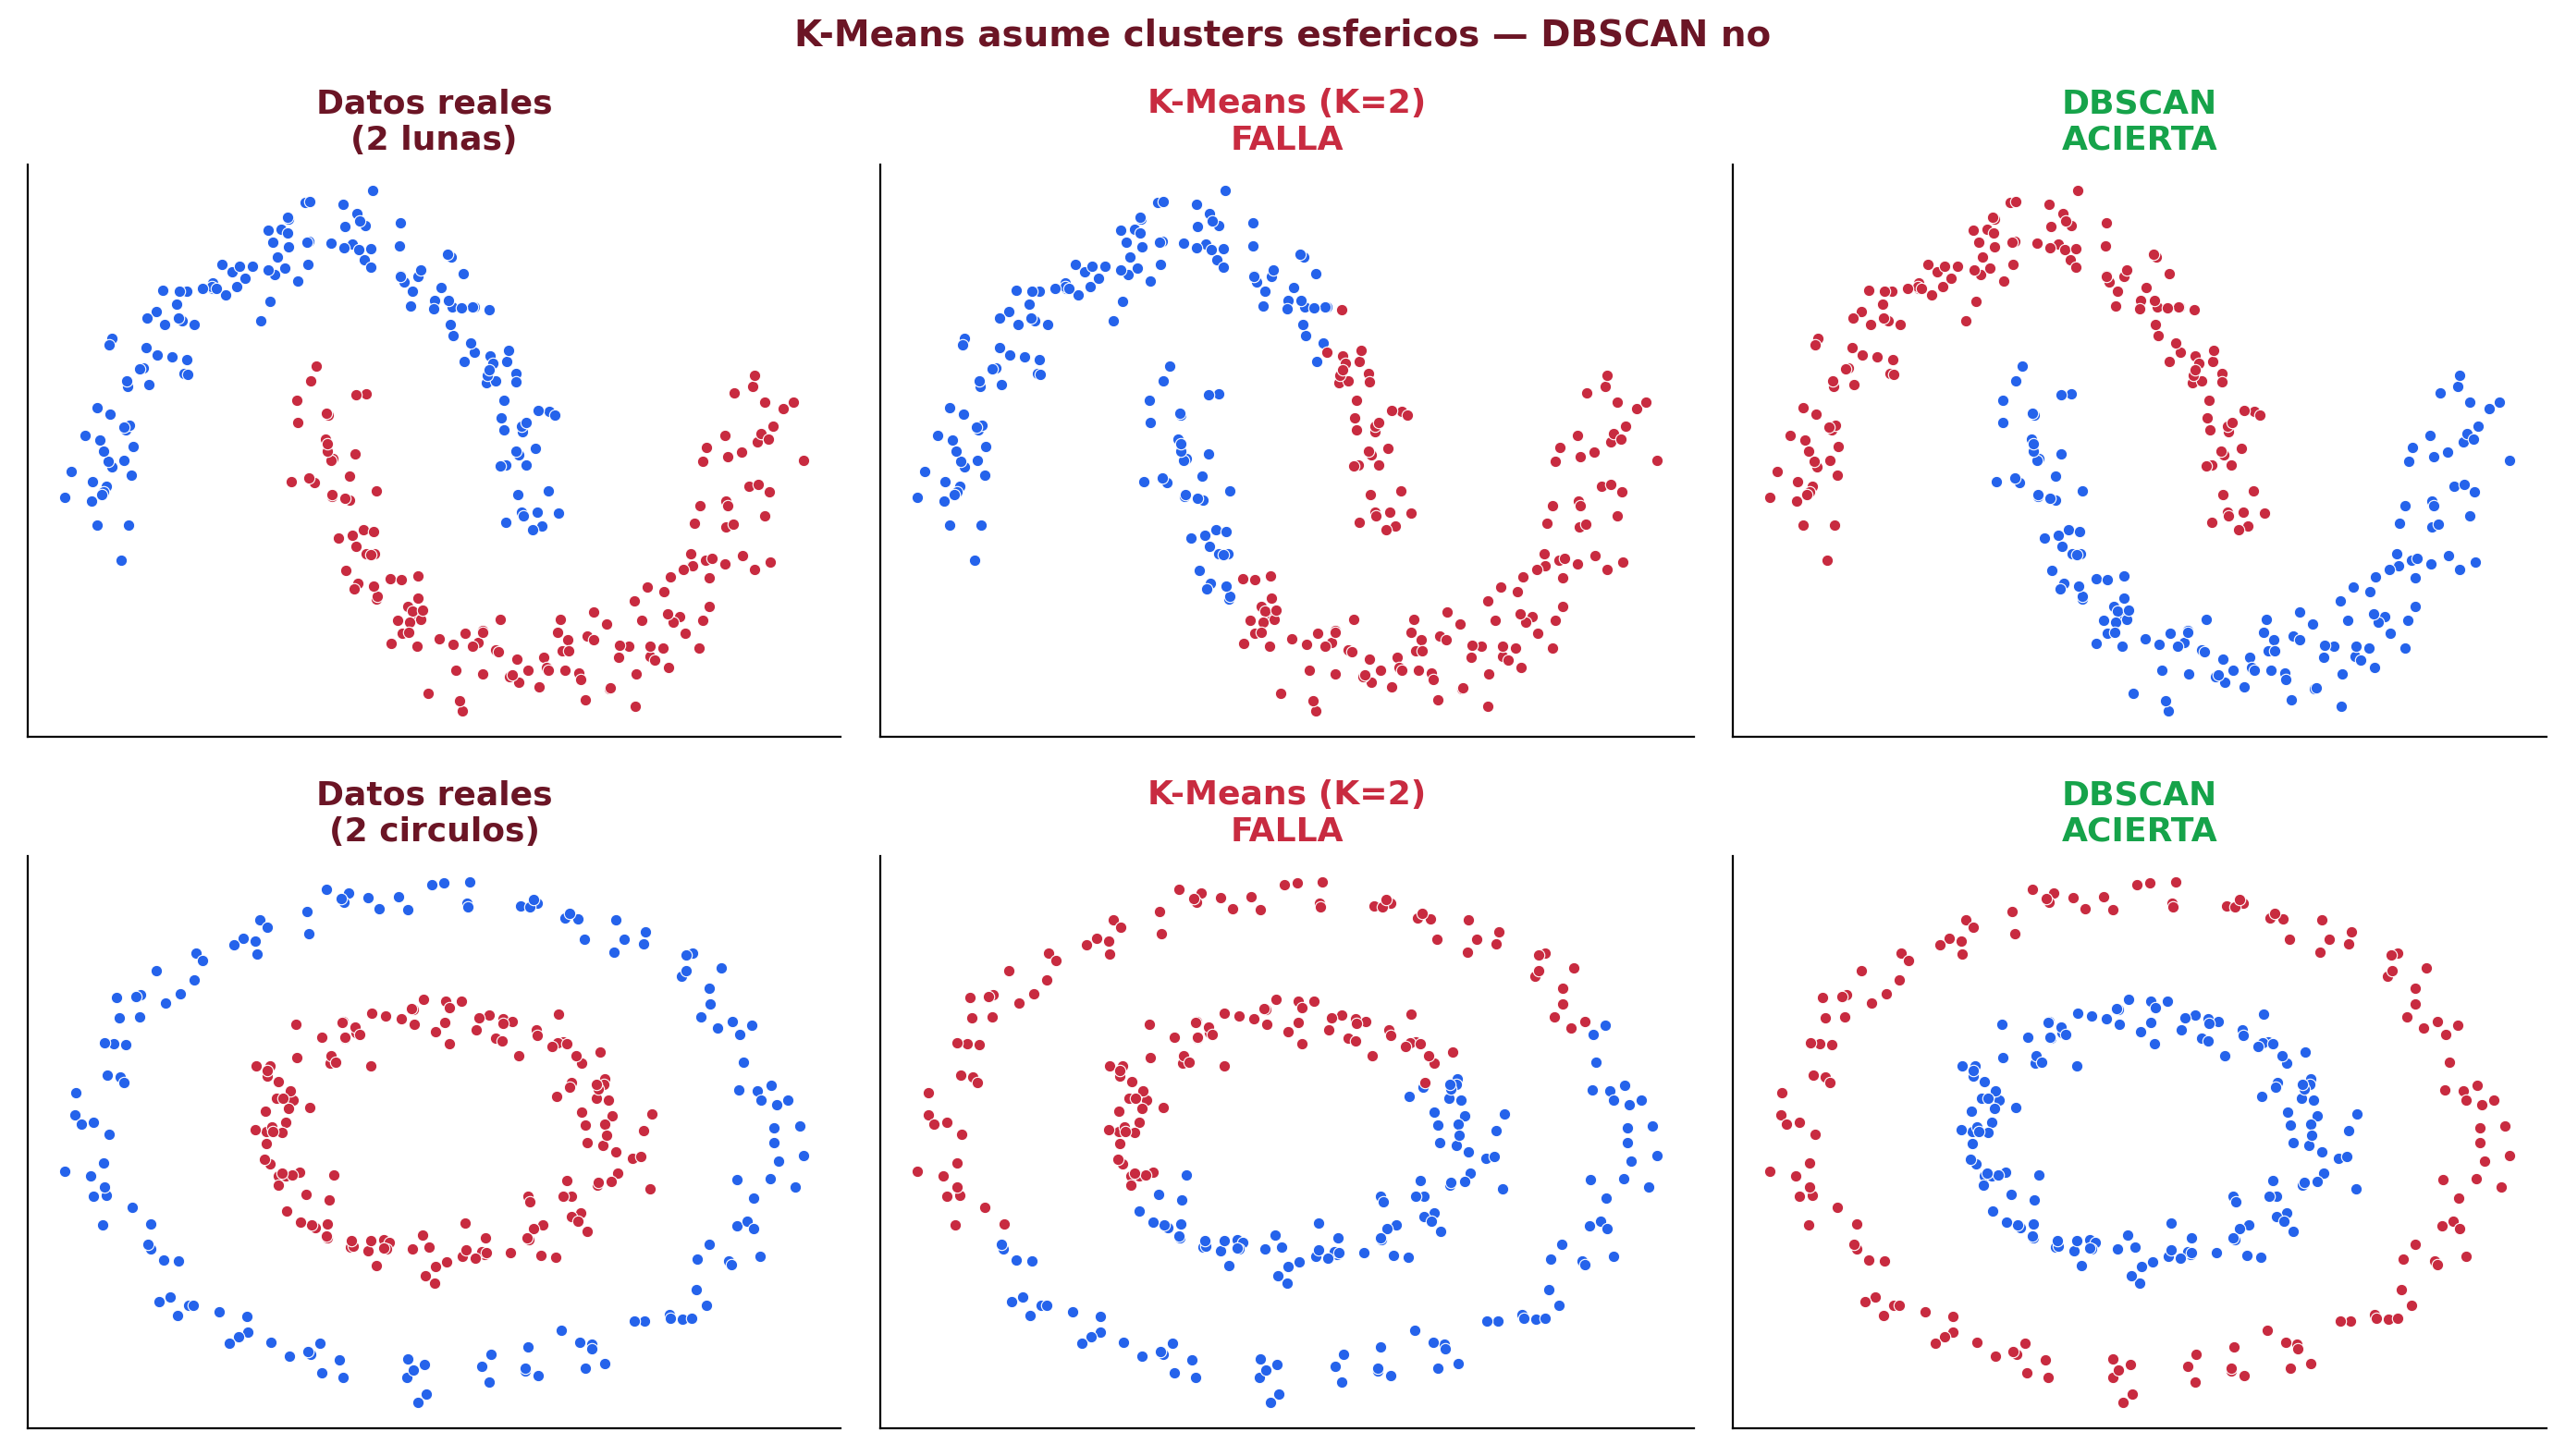
\includegraphics[width=0.92\textwidth]{fig_kmeans_falla.png}
  \end{center}

  \vspace{-2pt}
  {\scriptsize\color{textMuted}
    \faLightbulb\hspace{4pt} \textbf{Fila 1:} dos lunas entrelazadas.
    K-Means corta vertical. DBSCAN sigue la forma.
    \textbf{Fila 2:} dos c\'irculos conc\'entricos.
    K-Means corta horizontal. DBSCAN los separa perfecto.}
\end{frame}

\begin{frame}{DBSCAN: La Idea en 30 Segundos}
  \vspace{-4pt}
  {\footnotesize\color{arcaDark}\bfseries
    DBSCAN = \textbf{D}ensity-\textbf{B}ased \textbf{S}patial
    \textbf{C}lustering of \textbf{A}pplications with \textbf{N}oise.
    Agrupa puntos que est\'an \textbf{juntos} (densos) y marca
    los aislados como \textbf{ruido}.}

  \vspace{6pt}
  {\footnotesize
  \begin{itemize}\setlength{\itemsep}{5pt}
    \item[{\color{arcaRed}\scriptsize\faArrowRight}]
      \textbf{eps}: radio del vecindario. ``?`Qu\'e tan cerca
      deben estar dos puntos para ser vecinos?''
    \item[{\color{arcaRed}\scriptsize\faArrowRight}]
      \textbf{min\_samples}: m\'inimo de vecinos para ser un
      \textbf{punto central} (core point). Si un punto tiene
      suficientes vecinos dentro de eps, es central y ``crece''
      el cluster a su alrededor.
    \item[{\color{codeGreen}\scriptsize\faCheckCircle}]
      Puntos que no est\'an cerca de nadie $\to$ etiqueta $-1$
      (\textbf{ruido / outlier}).
  \end{itemize}
  }

  \vspace{4pt}
  \begin{tcolorbox}[colback=arcaGray, colframe=arcaRed, boxrule=0.5pt, arc=2pt,
    left=6pt, right=6pt, top=4pt, bottom=4pt]
    {\scriptsize\color{arcaDark}
    \faKey\hspace{4pt}\textbf{No necesita K.} DBSCAN descubre
    cu\'antos clusters hay solo. Y si un punto es raro, lo dice.}
  \end{tcolorbox}
\end{frame}

\begin{frame}[shrink=18]{DBSCAN: eps y min\_samples --- Visual}
  \vspace{-4pt}
  \begin{center}
    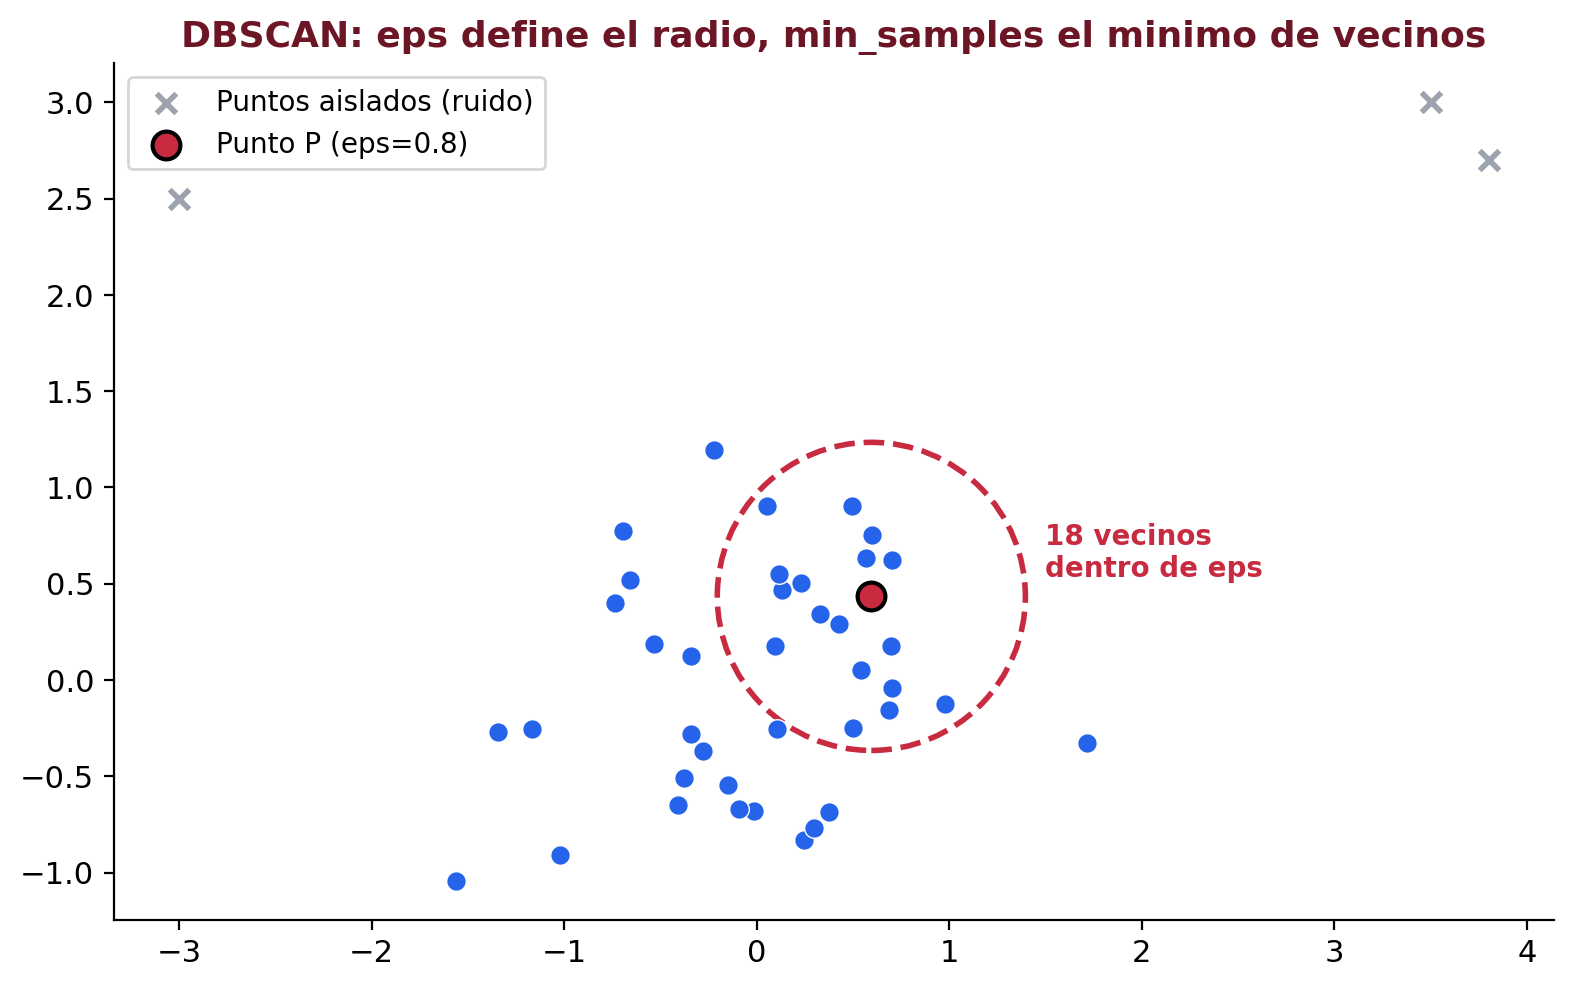
\includegraphics[width=0.68\textwidth]{fig_dbscan_concepto.png}
  \end{center}

  \vspace{-2pt}
  {\scriptsize\color{textMuted}
    \faLightbulb\hspace{4pt} El c\'irculo rojo es el radio \texttt{eps}
    alrededor de un punto. Si tiene suficientes vecinos dentro
    ($\geq$ \texttt{min\_samples}), es un \textbf{core point} y ``contagia''
    su cluster a los vecinos. Los puntos aislados (X grises) son ruido.}
\end{frame}

\begin{frame}[shrink=5]{K-Means vs DBSCAN --- Comparaci\'on}
  \vspace{-4pt}
  {\scriptsize
  \begin{tabular}{@{}p{3cm}p{4.5cm}p{4.5cm}@{}}
    \toprule
     & \textbf{\color{codeBlue}K-Means} & \textbf{\color{codeGreen}DBSCAN} \\
    \midrule
    \textbf{Forma de clusters} & Esf\'ericos (``bolitas''). & Cualquier forma. \\
    \textbf{N\'umero de clusters} & T\'u eliges $K$. & Lo descubre solo. \\
    \textbf{Outliers} & No los detecta (todos asignados). & Los marca como $-1$ (ruido). \\
    \textbf{Par\'ametros} & \texttt{n\_clusters} & \texttt{eps}, \texttt{min\_samples} \\
    \textbf{Escalabilidad} & R\'apido (millones). & M\'as lento con muchos datos. \\
    \textbf{Datos nuevos} & \texttt{.predict()} funciona. & \textbf{No tiene} \texttt{.predict()}. \\
    \textbf{Cu\'ando usarlo} & Clusters compactos, separados. & Formas irregulares, detectar anomal\'ias. \\
    \bottomrule
  \end{tabular}
  }

  \vspace{6pt}
  \begin{tcolorbox}[colback=codeGreen!8, colframe=codeGreen, boxrule=0.5pt, arc=2pt,
    left=6pt, right=6pt, top=4pt, bottom=4pt]
    {\scriptsize\color{arcaDark}
    \faKey\hspace{4pt}\textbf{No son competidores, son complementarios.}
    En segmentaci\'on de clientes (formas esf\'ericas), K-Means
    suele ganar. En detecci\'on de anomal\'ias o datos con formas
    irregulares, DBSCAN es superior.}
  \end{tcolorbox}
\end{frame}

\begin{frame}[fragile,shrink=10]{C\'odigo: DBSCAN en 4 L\'ineas}
  \vspace{-4pt}
  \begin{pyblock}
from sklearn.cluster import DBSCAN

db = DBSCAN(eps=0.45, min_samples=5)
labels = db.fit_predict(X_scaled)

n_clusters = len(set(labels) - {-1})
n_ruido = (labels == -1).sum()
print(f"Clusters: {n_clusters}, Ruido: {n_ruido}")
  \end{pyblock}

  \vspace{4pt}
  {\scriptsize\color{arcaDark}
  \begin{itemize}\setlength{\itemsep}{3pt}
    \item[{\color{arcaRed}\scriptsize\faArrowRight}]
      \texttt{labels = -1} significa \textbf{ruido} (outlier).
    \item[{\color{arcaRed}\scriptsize\faArrowRight}]
      No hay \texttt{n\_clusters}: DBSCAN lo decide solo.
    \item[{\color{codeGreen}\scriptsize\faArrowRight}]
      \texttt{eps} y \texttt{min\_samples} se ajustan probando.
      Un \texttt{eps} muy chico = todo es ruido.
      Un \texttt{eps} muy grande = todo es un solo cluster.
  \end{itemize}
  }
\end{frame}

\begin{frame}[shrink=18]{K-Means vs DBSCAN en Mall Customers}
  \vspace{-4pt}
  \begin{center}
    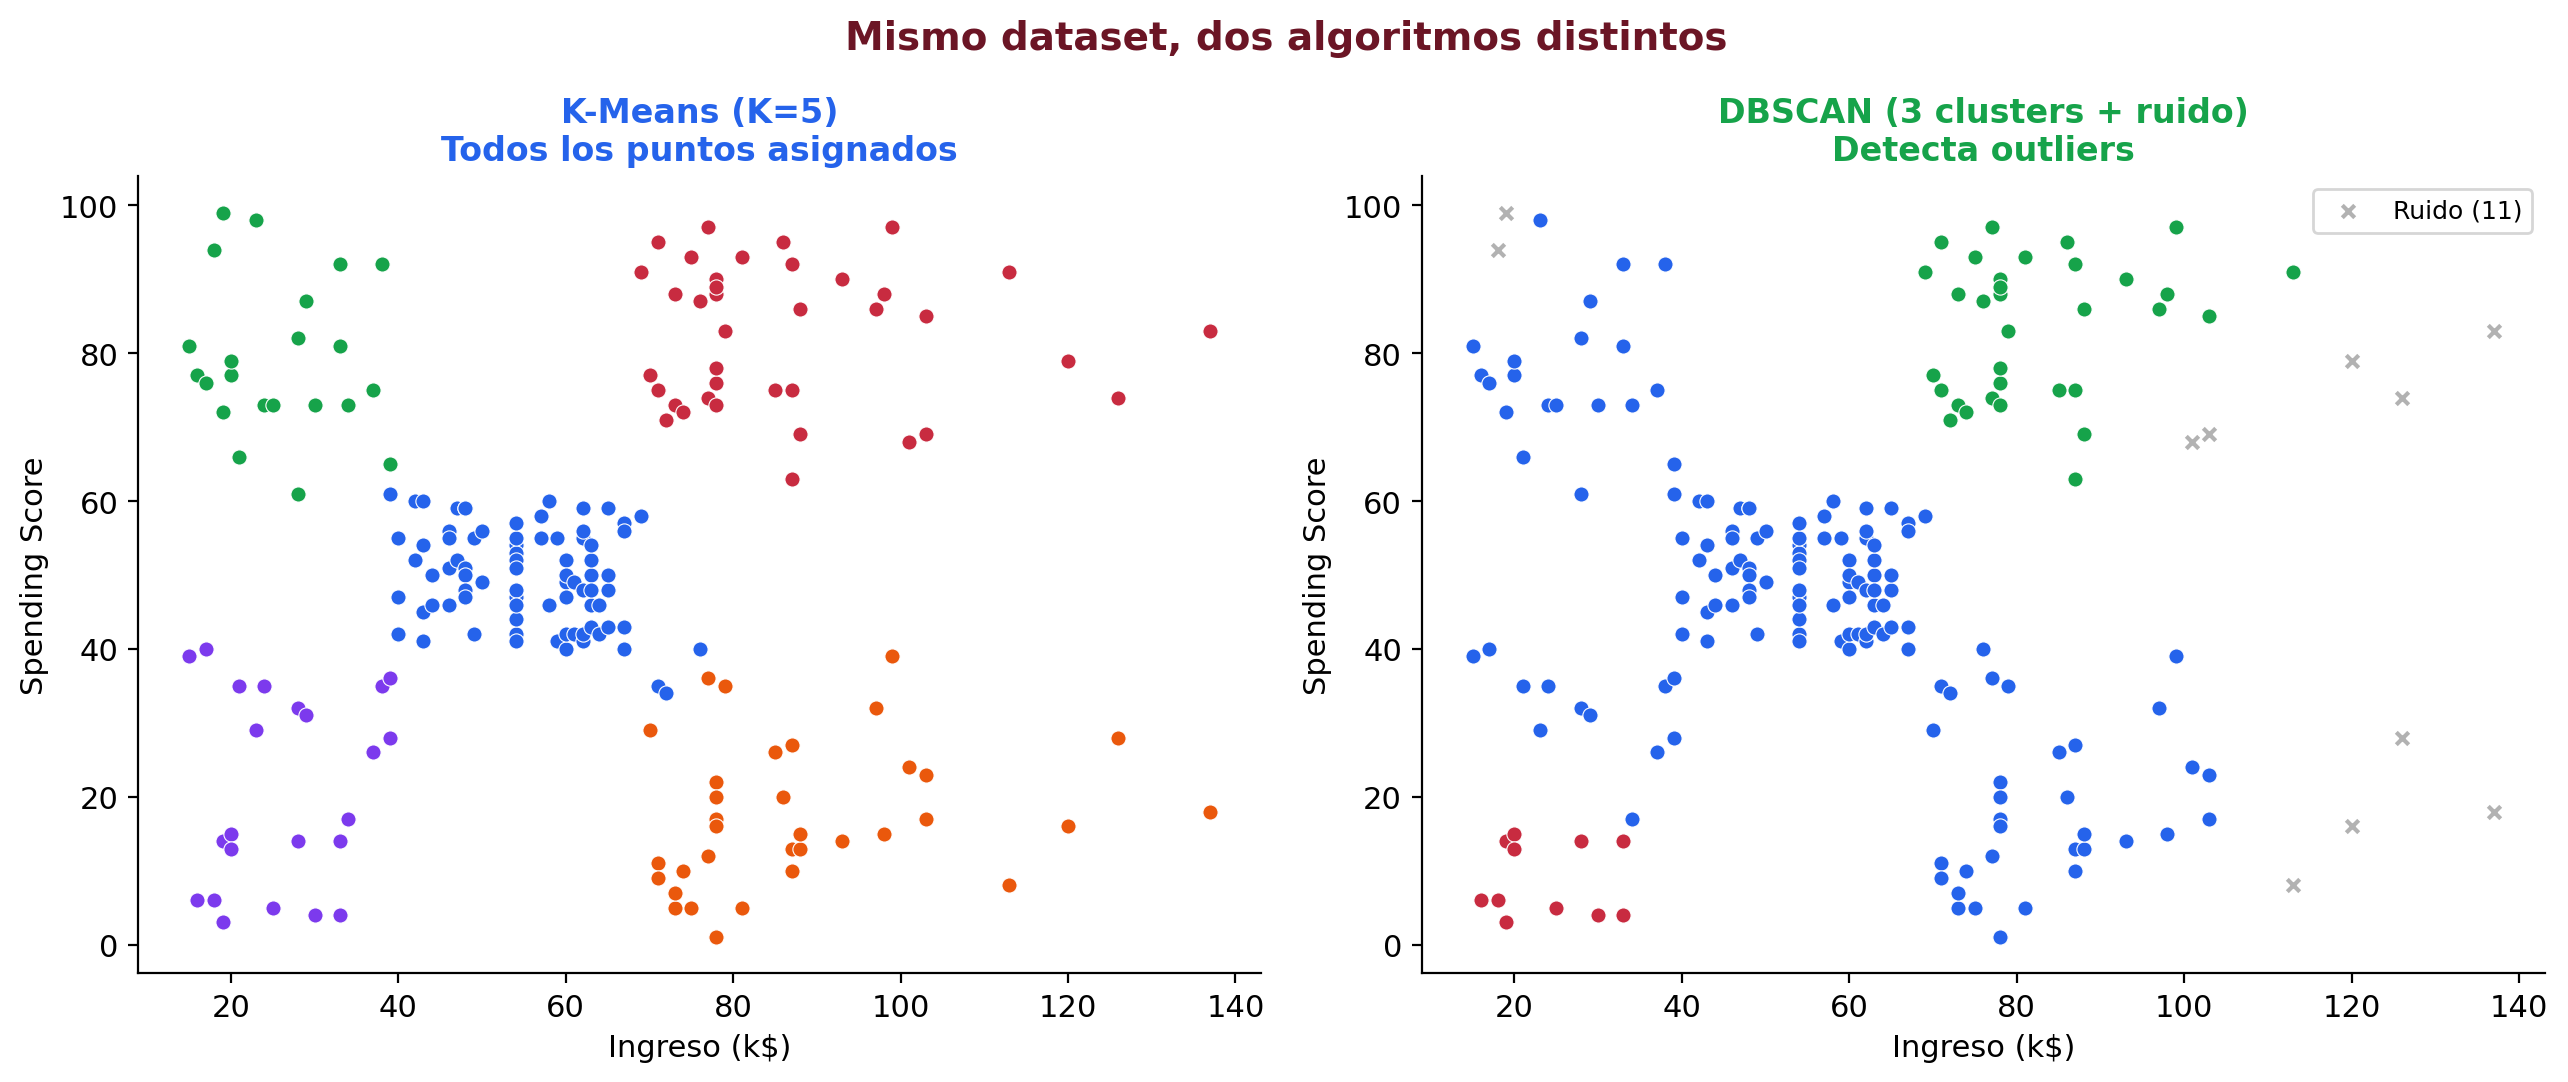
\includegraphics[width=0.88\textwidth]{fig_kmeans_vs_dbscan.png}
  \end{center}

  \vspace{-2pt}
  {\scriptsize\color{textMuted}
    \faLightbulb\hspace{4pt} \textbf{Izquierda:} K-Means asigna todos
    los puntos, incluidos los at\'ipicos.
    \textbf{Derecha:} DBSCAN detecta los puntos fronterizos como ruido
    (X grises). Para segmentaci\'on de clientes, ambos son v\'alidos ---
    depende de si queremos detectar outliers o no.}
\end{frame}

% =============================================================================
%  BLOQUE C2: Y EL CLIENTE NUEVO?
% =============================================================================
\sectionframe{?`Y el Cliente Nuevo?}{De clustering a clasificaci\'on}

\begin{frame}{El Problema: Llega un Cliente Nuevo al Mall}
  \vspace{-4pt}
  {\footnotesize\color{arcaDark}\bfseries
    Entrenamos K-Means, encontramos 5 segmentos, le dimos nombres,
    hicimos estrategias. Lunes llega un cliente nuevo.
    ?`A qu\'e segmento pertenece?}

  \vspace{6pt}
  {\footnotesize
  \begin{itemize}\setlength{\itemsep}{5pt}
    \item[{\color{codeGreen}\scriptsize\faCheckCircle}]
      \textbf{K-Means s\'i tiene} \texttt{.predict()}: calcula la
      distancia del nuevo punto a los 5 centroides y lo asigna al
      m\'as cercano. Funciona directo.
    \item[{\color{arcaRed}\scriptsize\faTimesCircle}]
      \textbf{DBSCAN no tiene} \texttt{.predict()}: una vez entrenado,
      no puede clasificar datos nuevos. ?`Qu\'e hacemos?
    \item[{\color{codeBlue}\scriptsize\faArrowRight}]
      \textbf{Soluci\'on general}: usar los clusters como
      \textbf{etiquetas} ($y$) y entrenar un clasificador supervisado
      encima. Ahora s\'i podemos predecir nuevos clientes.
  \end{itemize}
  }

  \vspace{4pt}
  \begin{tcolorbox}[colback=codePurple!8, colframe=codePurple, boxrule=0.5pt, arc=2pt,
    left=6pt, right=6pt, top=4pt, bottom=4pt]
    {\scriptsize\color{arcaDark}
    \faLightbulb\hspace{4pt}\textbf{Esto conecta todo el diplomado:}
    primero descubrimos los grupos (no supervisado), luego
    entrenamos un modelo para predecirlos (supervisado).
    Clustering $\to$ feature engineering $\to$ clasificaci\'on.}
  \end{tcolorbox}
\end{frame}

\begin{frame}[fragile,shrink=18]{Opci\'on 1: \texttt{km.predict()} --- La V\'ia R\'apida}
  \vspace{-4pt}
  {\footnotesize\color{arcaDark}\bfseries
    Si usamos K-Means, ya tenemos \texttt{.predict()} gratis:}

  \vspace{4pt}
  \begin{pyblock}
# Cliente nuevo: ingreso 70k, gasto 85
nuevo = [[70, 85]]
segmento = km.predict(nuevo)
print(f"Segmento: {nombres[segmento[0]]}")
# -> "Premium"
  \end{pyblock}

  \vspace{4pt}
  {\scriptsize\color{arcaDark}
    \faCheckCircle\hspace{4pt} Simple. Pero solo funciona con K-Means.
    Si usamos DBSCAN, o si queremos usar variables que no estaban en
    el clustering (ej. g\'enero), necesitamos otra cosa.}
\end{frame}

\begin{frame}[fragile,shrink=22]{Opci\'on 2: Clasificador Encima --- La V\'ia General}
  \vspace{-6pt}
  {\footnotesize\color{arcaDark}\bfseries
    Usamos los clusters como target y entrenamos un modelo supervisado:}

  \vspace{4pt}
  \begin{pyblock}
from sklearn.ensemble import RandomForestClassifier
from sklearn.model_selection import cross_val_score

# 1. Los clusters descubiertos son ahora nuestro "y"
y_segmentos = df["cluster"]

# 2. Entrenar un clasificador con TODAS las variables
X_clf = df[["Age", "income", "spending"]]
clf = RandomForestClassifier(n_estimators=100, random_state=42)
clf.fit(X_clf, y_segmentos)

# 3. Predecir cliente nuevo
nuevo = pd.DataFrame([{"Age": 28, "income": 70, "spending": 85}])
pred = clf.predict(nuevo)
print(f"Segmento: {nombres[pred[0]]}")
  \end{pyblock}

  \vspace{2pt}
  {\scriptsize\color{arcaDark}
    \faKey\hspace{4pt} Ventajas: funciona con cualquier algoritmo de
    clustering, puede usar variables extra (g\'enero, ciudad),
    y se puede meter dentro de un \textbf{Pipeline}.}
\end{frame}

% =============================================================================
%  BLOQUE D: EJERCICIO IRIS
% =============================================================================
\sectionframe{Ejercicio: Iris}{Descubrir especies sin etiquetas}

\begin{frame}[shrink=5]{Ejercicio 3: Descubrir Especies Sin Etiquetas}
  \vspace{-4pt}
  {\footnotesize\color{arcaDark}\bfseries
    \faClock\hspace{4pt} 15 minutos --- un bi\'ologo te da mediciones
    de 150 flores. 4 medidas por flor. \textbf{No sabe cu\'antas
    especies hay.}}

  \vspace{6pt}
  {\footnotesize
  \begin{enumerate}\setlength{\itemsep}{4pt}
    \item Cargar: \texttt{from sklearn.datasets import load\_iris}
    \item Usar \textbf{solo} \texttt{iris.data} (las medidas).
      \textbf{No mirar} \texttt{iris.target}.
    \item Escalar con \texttt{StandardScaler}.
    \item M\'etodo del codo + Silhouette. ?`Cu\'antos clusters sugieren?
    \item K-Means con ese K. Scatter: \texttt{petal length} vs
      \texttt{petal width}, coloreado por cluster.
    \item \textbf{Revelar:} \texttt{pd.crosstab(cluster, iris.target)}.
      ?`K-Means recuper\'o las 3 especies?
  \end{enumerate}
  }

  \vspace{4pt}
  {\scriptsize\color{textMuted}
    \faLightbulb\hspace{4pt} Setosa siempre se separa perfectamente.
    Versicolor y Virginica se confunden un poco --- esas dos especies
    son parecidas en sus medidas.}
\end{frame}

% =============================================================================
%  BLOQUE D: PIPELINES
% =============================================================================
\sectionframe{Pipelines de sklearn}{Encadenar pasos sin errores}

\begin{frame}{El Problema: Pasos Sueltos}
  \vspace{-4pt}
  {\footnotesize\color{arcaDark}\bfseries
    Hasta ahora hac\'iamos el preprocesamiento y el modelo por separado:}

  \vspace{6pt}
  {\footnotesize
  \begin{enumerate}\setlength{\itemsep}{3pt}
    \item[{\color{arcaRed}\bfseries 1.}]
      \texttt{scaler.fit\_transform(X\_train)} ---
      \texttt{scaler.transform(X\_test)}
    \item[{\color{arcaRed}\bfseries 2.}]
      \texttt{modelo.fit(X\_train\_s, y\_train)}
    \item[{\color{arcaRed}\bfseries 3.}]
      \texttt{modelo.predict(X\_test\_s)}
  \end{enumerate}
  }

  \vspace{6pt}
  {\footnotesize\bfseries\color{arcaRed} Dos problemas:}

  \vspace{4pt}
  {\footnotesize
  \begin{itemize}\setlength{\itemsep}{4pt}
    \item[{\color{arcaRed}\scriptsize\faTimesCircle}]
      \textbf{F\'acil olvidar un paso} --- si olvidas escalar X\_test,
      el modelo recibe datos en otra escala y predice basura.
    \item[{\color{arcaRed}\scriptsize\faTimesCircle}]
      \textbf{Data leakage} --- si haces \texttt{fit\_transform(X)}
      antes del split, el scaler ``ve'' datos de test.
  \end{itemize}
  }

  \vspace{4pt}
  {\scriptsize\color{textMuted}
    \faArrowRight\hspace{4pt} \textbf{Pipeline resuelve ambos problemas}:
    encadena los pasos en un solo objeto.}
\end{frame}

\begin{frame}[shrink=18]{Sin Pipeline vs Con Pipeline}
  \vspace{-4pt}
  \begin{center}
    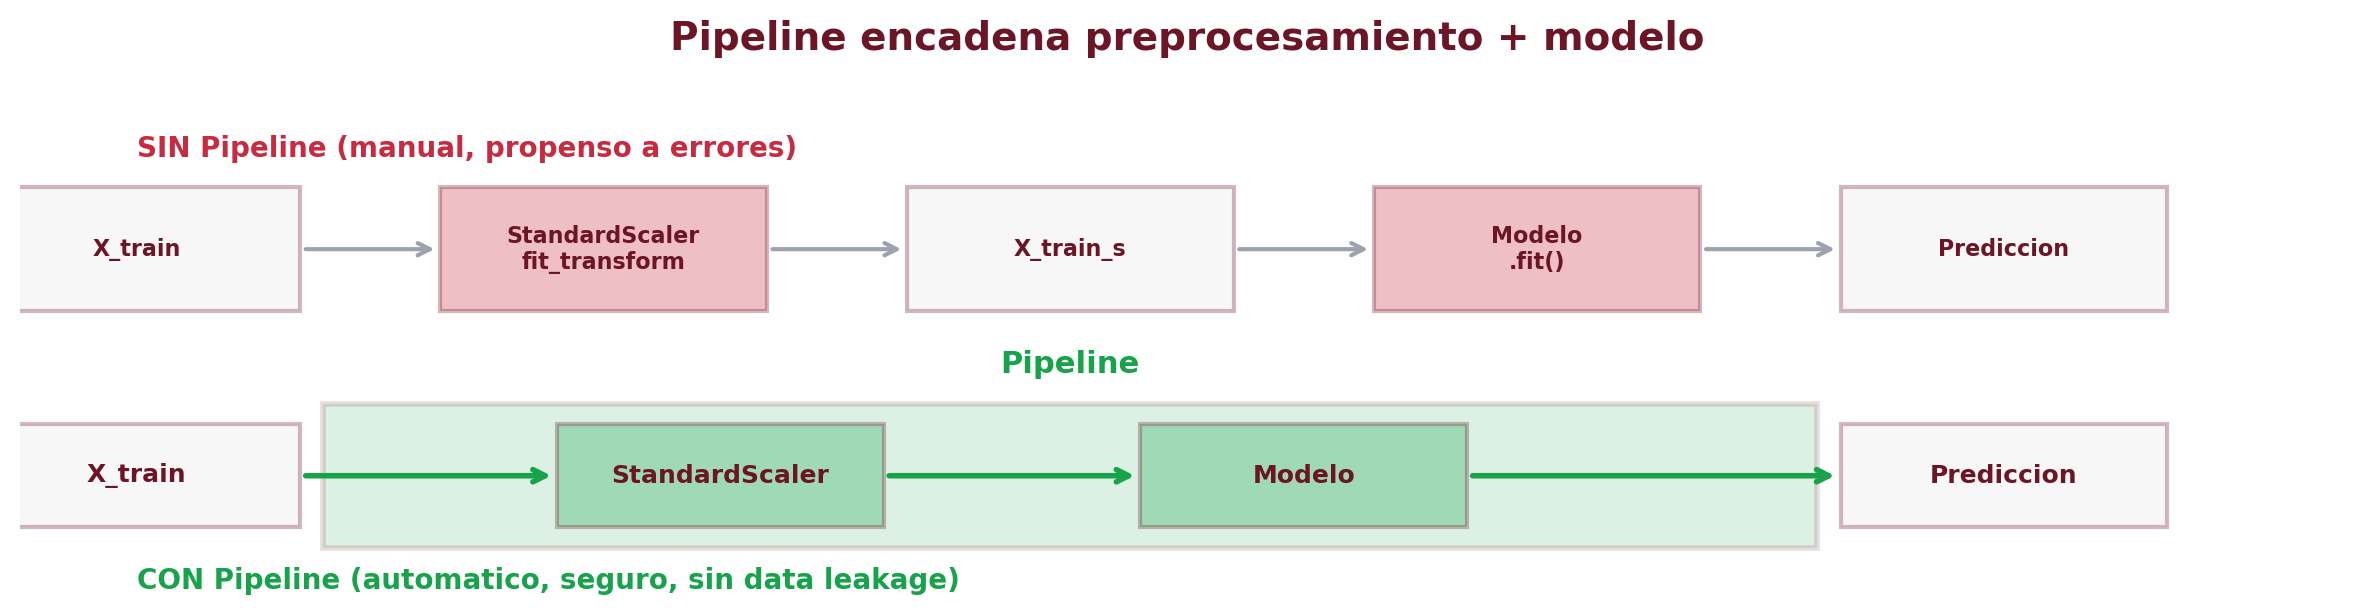
\includegraphics[width=0.88\textwidth]{fig_pipeline.png}
  \end{center}

  \vspace{-2pt}
  {\scriptsize\color{textMuted}
    \faLightbulb\hspace{4pt} Pipeline encadena StandardScaler + Modelo
    en un solo objeto. \texttt{fit()} escala y entrena.
    \texttt{predict()} escala y predice. Cero posibilidad de error.}
\end{frame}

\begin{frame}[fragile,shrink=18]{C\'odigo: Tu Primer Pipeline}
  \vspace{-6pt}
  \begin{pyblock}
from sklearn.pipeline import Pipeline
from sklearn.linear_model import LogisticRegression

# CON Pipeline: mismo resultado, menos codigo, sin errores
pipe_lr = Pipeline([
    ("scaler", StandardScaler()),
    ("modelo", LogisticRegression(max_iter=1000,
        class_weight="balanced", random_state=42))
])

# Un solo .fit() escala Y entrena
pipe_lr.fit(X_train, y_train)

# Un solo .predict_proba() escala Y predice
y_prob = pipe_lr.predict_proba(X_test)[:, 1]
print(f"AUC: {roc_auc_score(y_test, y_prob):.3f}")
  \end{pyblock}

  \vspace{4pt}
  {\scriptsize\color{arcaDark}
    \faKey\hspace{4pt} Cada paso tiene un \textbf{nombre} (``scaler'',
    ``modelo'') y un \textbf{estimador}. El Pipeline los ejecuta en
    orden.}
\end{frame}

\begin{frame}[shrink=18]{Data Leakage: Por Qu\'e Pipeline Importa}
  \vspace{-4pt}
  \begin{center}
    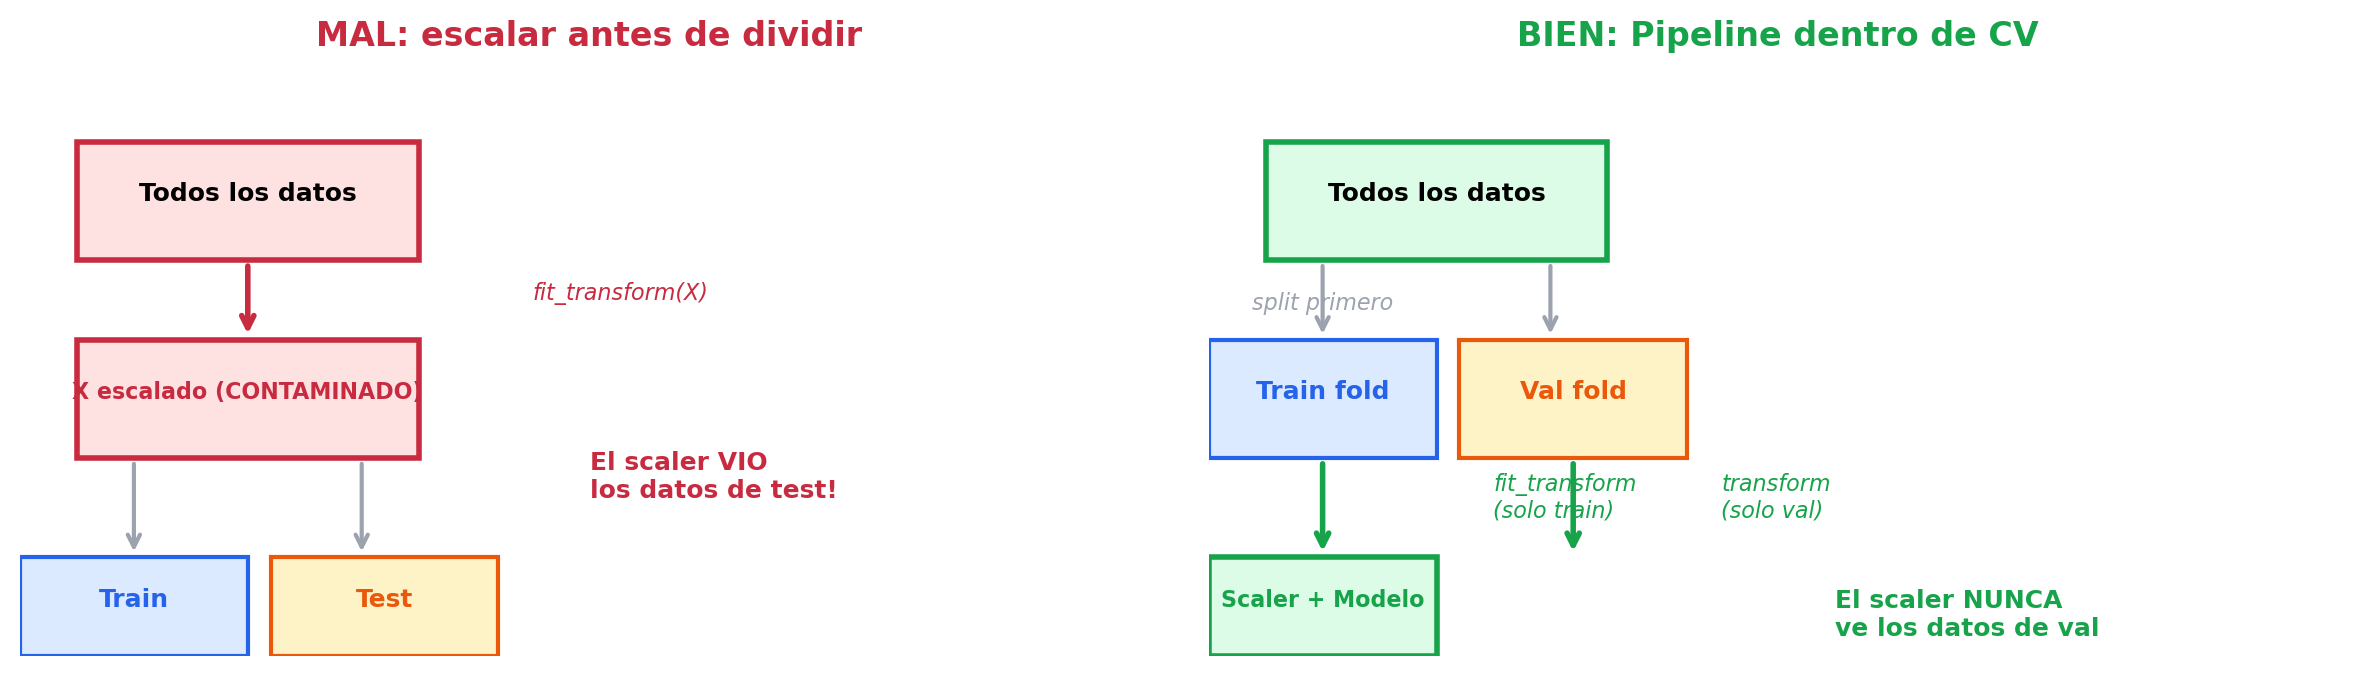
\includegraphics[width=0.88\textwidth]{fig_data_leakage.png}
  \end{center}

  \vspace{-2pt}
  {\scriptsize\color{textMuted}
    \faLightbulb\hspace{4pt} \textbf{Izquierda:} escalar antes de dividir
    contamina. El scaler ``ve'' los datos de test.
    \textbf{Derecha:} Pipeline dentro de CV divide primero, escala
    despu\'es. Cada fold es independiente.}
\end{frame}

\begin{frame}[fragile,shrink=10]{Pipeline + Cross-Validation}
  \vspace{-4pt}
  {\footnotesize\color{arcaDark}\bfseries
    Cuando usamos Pipeline dentro de \texttt{cross\_val\_score},
    el scaler se ajusta \textbf{solo en los folds de train}:}

  \vspace{4pt}
  \begin{pyblock}
from sklearn.model_selection import cross_val_score

scores = cross_val_score(pipe_lr, X_train, y_train,
                         cv=5, scoring="roc_auc")
print(f"AUC: {scores.mean():.3f} +/- {scores.std():.3f}")
  \end{pyblock}

  \vspace{4pt}
  {\scriptsize\color{arcaDark}
  En cada fold, el Pipeline:
  \begin{enumerate}\setlength{\itemsep}{2pt}
    \item[{\color{arcaRed}\bfseries 1.}]
      Ajusta el scaler en los 4 folds de train $\to$ \texttt{fit\_transform}
    \item[{\color{arcaRed}\bfseries 2.}]
      Transforma el fold de validaci\'on $\to$ \texttt{transform} (sin fit!)
    \item[{\color{arcaRed}\bfseries 3.}]
      Entrena el modelo en datos escalados de train
    \item[{\color{arcaRed}\bfseries 4.}]
      Eval\'ua en datos escalados de validaci\'on
  \end{enumerate}
  }
\end{frame}

\begin{frame}[shrink=18]{Pipeline + GridSearchCV: Notaci\'on}
  \vspace{-4pt}
  \begin{center}
    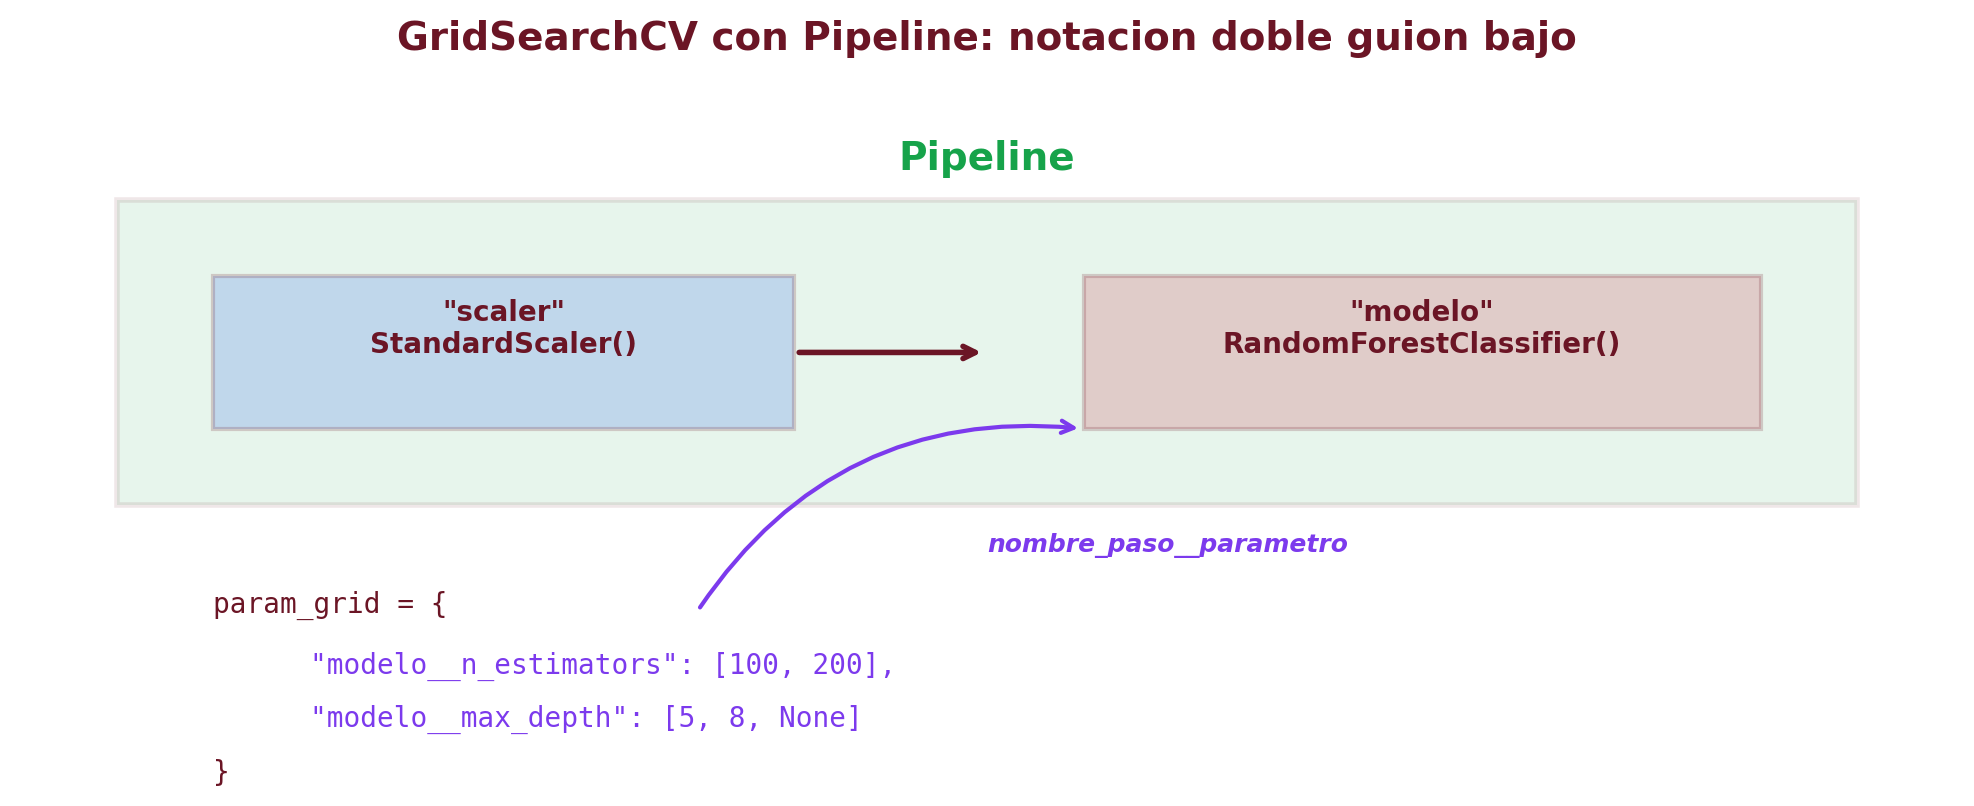
\includegraphics[width=0.78\textwidth]{fig_gridsearch_pipeline.png}
  \end{center}

  \vspace{-2pt}
  {\scriptsize\color{textMuted}
    \faLightbulb\hspace{4pt} Los par\'ametros del grid usan la notaci\'on
    \texttt{nombre\_paso\_\_parametro} (doble guion bajo).
    Ejemplo: \texttt{modelo\_\_n\_estimators} accede al par\'ametro
    \texttt{n\_estimators} del paso ``modelo''.}
\end{frame}

\begin{frame}[fragile,shrink=18]{C\'odigo: GridSearchCV con Pipeline}
  \vspace{-6pt}
  \begin{pyblock}
from sklearn.model_selection import GridSearchCV
from sklearn.ensemble import RandomForestClassifier

pipe_rf = Pipeline([
    ("scaler", StandardScaler()),
    ("modelo", RandomForestClassifier(
        class_weight="balanced", random_state=42))
])

param_grid = {
    "modelo__n_estimators": [100, 200],
    "modelo__max_depth": [5, 8, None],
}

grid = GridSearchCV(pipe_rf, param_grid,
                    cv=5, scoring="roc_auc", n_jobs=-1)
grid.fit(X_train, y_train)
print(f"Mejor AUC: {grid.best_score_:.3f}")
print(f"Params: {grid.best_params_}")
  \end{pyblock}
\end{frame}

\begin{frame}{Pipeline para Clustering}
  \vspace{-4pt}
  {\footnotesize\color{arcaDark}\bfseries
    Pipelines no son solo para clasificaci\'on --- tambi\'en funcionan
    con K-Means:}

  \vspace{6pt}
  {\footnotesize
  \begin{itemize}\setlength{\itemsep}{5pt}
    \item[{\color{codeGreen}\scriptsize\faCheckCircle}]
      \texttt{Pipeline([("scaler", StandardScaler()),
      ("kmeans", KMeans(n\_clusters=5))])}
    \item[{\color{codeGreen}\scriptsize\faCheckCircle}]
      \texttt{pipe.fit\_predict(datos)} escala y agrupa en una sola l\'inea.
    \item[{\color{codeGreen}\scriptsize\faCheckCircle}]
      Si cambias \texttt{StandardScaler} por \texttt{MinMaxScaler},
      solo modificas una l\'inea.
  \end{itemize}
  }

  \vspace{6pt}
  \begin{tcolorbox}[colback=codeGreen!8, colframe=codeGreen, boxrule=0.5pt, arc=2pt,
    left=6pt, right=6pt, top=4pt, bottom=4pt]
    {\scriptsize\color{arcaDark}
    \faKey\hspace{4pt}\textbf{De ahora en adelante:} siempre usar Pipelines.
    Es la forma profesional de trabajar en ML. Previene errores,
    previene data leakage, y hace el c\'odigo m\'as limpio.}
  \end{tcolorbox}
\end{frame}

\begin{frame}[shrink=5]{Ejercicio 4: Pipeline con DecisionTree}
  \vspace{-4pt}
  {\footnotesize\color{arcaDark}\bfseries
    \faClock\hspace{4pt} 10 minutos:}

  \vspace{6pt}
  {\footnotesize
  \begin{enumerate}\setlength{\itemsep}{4pt}
    \item Crea un Pipeline con \texttt{StandardScaler} +
      \texttt{DecisionTreeClassifier(max\_depth=5)}.
    \item Eval\'ua con \texttt{cross\_val\_score}
      (cv=5, scoring=``roc\_auc'') en diabetes.
    \item Compara su AUC con Log\'istica y Random Forest.
    \item \textbf{Pregunta:} ?`tiene sentido que el \'arbol tenga
      el scaler? ?`Lo necesita?
  \end{enumerate}
  }

  \vspace{6pt}
  {\scriptsize\color{textMuted}
    \faLightbulb\hspace{4pt} Los \'arboles no se ven afectados por la
    escala (usan splits, no distancias). El scaler no perjudica
    pero no es necesario. En un Pipeline mixto es c\'omodo tenerlo.}
\end{frame}

% =============================================================================
%  CIERRE
% =============================================================================
\sectionframe{Cierre}{Lo que aprendimos hoy}

\begin{frame}[shrink=10]{Resumen}
  \vspace{-4pt}
  \begin{columns}[T]
    \begin{column}{0.48\textwidth}
      {\footnotesize\bfseries\color{arcaRed} Clustering:}
      \vspace{4pt}

      {\footnotesize
      \begin{itemize}\setlength{\itemsep}{3pt}
        \item[{\color{codeGreen}\faCheckCircle}]
          Perfilar + nombrar segmentos.
        \item[{\color{codeGreen}\faCheckCircle}]
          K-Means 3D + StandardScaler.
        \item[{\color{codeGreen}\faCheckCircle}]
          DBSCAN: formas irregulares + outliers.
        \item[{\color{codeGreen}\faCheckCircle}]
          K-Means $\neq$ DBSCAN: complementarios.
      \end{itemize}
      }

      \vspace{4pt}
      {\footnotesize\bfseries\color{codeBlue} Cliente nuevo:}
      \vspace{4pt}

      {\footnotesize
      \begin{itemize}\setlength{\itemsep}{3pt}
        \item[{\color{codeBlue}\faCheckCircle}]
          K-Means: \texttt{.predict()} directo.
        \item[{\color{codeBlue}\faCheckCircle}]
          DBSCAN: no tiene predict.
        \item[{\color{codeBlue}\faCheckCircle}]
          Soluci\'on: clasificador encima.
        \item[{\color{codeBlue}\faCheckCircle}]
          Clustering $\to$ clasificaci\'on.
      \end{itemize}
      }
    \end{column}

    \begin{column}{0.48\textwidth}
      {\footnotesize\bfseries\color{codeGreen} Pipelines:}
      \vspace{4pt}

      {\footnotesize
      \begin{itemize}\setlength{\itemsep}{3pt}
        \item[{\color{codeGreen}\faCheckCircle}]
          Encadena preprocesamiento + modelo.
        \item[{\color{codeGreen}\faCheckCircle}]
          Previene data leakage en CV.
        \item[{\color{codeGreen}\faCheckCircle}]
          GridSearchCV: \texttt{paso\_\_param}.
        \item[{\color{codeGreen}\faCheckCircle}]
          \textbf{Forma profesional} de hacer ML.
      \end{itemize}
      }
    \end{column}
  \end{columns}

  \vspace{6pt}
  \begin{tcolorbox}[colback=arcaRed!8, colframe=arcaRed, boxrule=0.5pt, arc=2pt,
    left=6pt, right=6pt, top=4pt, bottom=4pt]
    {\scriptsize\color{arcaDark}
    \faArrowRight\hspace{4pt}\textbf{Pr\'oxima clase:} M\'odulo 4 ---
    Machine Learning Supervisado, No Supervisado y Segmentaci\'on.}
  \end{tcolorbox}
\end{frame}

% ── QR ENCUESTA ──────────────────────────────────────────────────────────────
{
\setbeamertemplate{headline}{}
\setbeamertemplate{footline}{}
\begin{frame}[plain, noframenumbering]
  \begin{tikzpicture}[remember picture, overlay]
    \fill[arcaDark] (current page.south west) rectangle (current page.north east);
  \end{tikzpicture}
  \vspace{1cm}
  \begin{center}
    {\Huge\bfseries\color{white} ?`C\'omo estuvo la clase?\par}
    \vspace{0.6cm}
    
\includegraphics[width=4cm]{qr_encuesta.jpg}
    \vspace{0.4cm}

    {\large\color{white!80} Escanea el QR para dejarnos tu opini\'on.\par}
  \end{center}
\end{frame}
}

\end{document}
